\documentclass[twoside]{book}

% Packages required by doxygen
\usepackage{calc}
\usepackage{doxygen}
\usepackage{graphicx}
\usepackage[utf8]{inputenc}
\usepackage{makeidx}
\usepackage{multicol}
\usepackage{multirow}
\usepackage{textcomp}
\usepackage[table]{xcolor}

% Font selection
\usepackage[T1]{fontenc}
\usepackage{mathptmx}
\usepackage[scaled=.90]{helvet}
\usepackage{courier}
\usepackage{amssymb}
\usepackage{sectsty}
\renewcommand{\familydefault}{\sfdefault}
\allsectionsfont{%
  \fontseries{bc}\selectfont%
  \color{darkgray}%
}
\renewcommand{\DoxyLabelFont}{%
  \fontseries{bc}\selectfont%
  \color{darkgray}%
}

% Page & text layout
\usepackage{geometry}
\geometry{%
  a4paper,%
  top=2.5cm,%
  bottom=2.5cm,%
  left=2.5cm,%
  right=2.5cm%
}
\tolerance=750
\hfuzz=15pt
\hbadness=750
\setlength{\emergencystretch}{15pt}
\setlength{\parindent}{0cm}
\setlength{\parskip}{0.2cm}
\makeatletter
\renewcommand{\paragraph}{%
  \@startsection{paragraph}{4}{0ex}{-1.0ex}{1.0ex}{%
    \normalfont\normalsize\bfseries\SS@parafont%
  }%
}
\renewcommand{\subparagraph}{%
  \@startsection{subparagraph}{5}{0ex}{-1.0ex}{1.0ex}{%
    \normalfont\normalsize\bfseries\SS@subparafont%
  }%
}
\makeatother

% Headers & footers
\usepackage{fancyhdr}
\pagestyle{fancyplain}
\fancyhead[LE]{\fancyplain{}{\bfseries\thepage}}
\fancyhead[CE]{\fancyplain{}{}}
\fancyhead[RE]{\fancyplain{}{\bfseries\leftmark}}
\fancyhead[LO]{\fancyplain{}{\bfseries\rightmark}}
\fancyhead[CO]{\fancyplain{}{}}
\fancyhead[RO]{\fancyplain{}{\bfseries\thepage}}
\fancyfoot[LE]{\fancyplain{}{}}
\fancyfoot[CE]{\fancyplain{}{}}
\fancyfoot[RE]{\fancyplain{}{\bfseries\scriptsize Generated on Wed Nov 27 2019 18\-:54\-:57 for Pirkamaan valloitus apjajoni by Doxygen }}
\fancyfoot[LO]{\fancyplain{}{\bfseries\scriptsize Generated on Wed Nov 27 2019 18\-:54\-:57 for Pirkamaan valloitus apjajoni by Doxygen }}
\fancyfoot[CO]{\fancyplain{}{}}
\fancyfoot[RO]{\fancyplain{}{}}
\renewcommand{\footrulewidth}{0.4pt}
\renewcommand{\chaptermark}[1]{%
  \markboth{#1}{}%
}
\renewcommand{\sectionmark}[1]{%
  \markright{\thesection\ #1}%
}

% Indices & bibliography
\usepackage{natbib}
\usepackage[titles]{tocloft}
\setcounter{tocdepth}{3}
\setcounter{secnumdepth}{5}
\makeindex

% Hyperlinks (required, but should be loaded last)
\usepackage{ifpdf}
\ifpdf
  \usepackage[pdftex,pagebackref=true]{hyperref}
\else
  \usepackage[ps2pdf,pagebackref=true]{hyperref}
\fi
\hypersetup{%
  colorlinks=true,%
  linkcolor=blue,%
  citecolor=blue,%
  unicode%
}

% Custom commands
\newcommand{\clearemptydoublepage}{%
  \newpage{\pagestyle{empty}\cleardoublepage}%
}


%===== C O N T E N T S =====

\begin{document}

% Titlepage & ToC
\hypersetup{pageanchor=false}
\pagenumbering{roman}
\begin{titlepage}
\vspace*{7cm}
\begin{center}%
{\Large Pirkamaan valloitus apjajoni }\\
\vspace*{1cm}
{\large Generated by Doxygen 1.8.5}\\
\vspace*{0.5cm}
{\small Wed Nov 27 2019 18:54:57}\\
\end{center}
\end{titlepage}
\clearemptydoublepage
\tableofcontents
\clearemptydoublepage
\pagenumbering{arabic}
\hypersetup{pageanchor=true}

%--- Begin generated contents ---
\chapter{Hierarchical Index}
\section{Class Hierarchy}
This inheritance list is sorted roughly, but not completely, alphabetically\-:\begin{DoxyCompactList}
\item \contentsline{section}{Course\-:\-:Coordinate}{\pageref{classCourse_1_1Coordinate}}{}
\item exception\begin{DoxyCompactList}
\item \contentsline{section}{Course\-:\-:Base\-Exception}{\pageref{classCourse_1_1BaseException}}{}
\begin{DoxyCompactList}
\item \contentsline{section}{Course\-:\-:Illegal\-Action}{\pageref{classCourse_1_1IllegalAction}}{}
\begin{DoxyCompactList}
\item \contentsline{section}{Course\-:\-:Not\-Enough\-Space}{\pageref{classCourse_1_1NotEnoughSpace}}{}
\item \contentsline{section}{Course\-:\-:Owner\-Conflict}{\pageref{classCourse_1_1OwnerConflict}}{}
\end{DoxyCompactList}
\item \contentsline{section}{Course\-:\-:Invalid\-Pointer}{\pageref{classCourse_1_1InvalidPointer}}{}
\item \contentsline{section}{Course\-:\-:Key\-Error}{\pageref{classCourse_1_1KeyError}}{}
\end{DoxyCompactList}
\end{DoxyCompactList}
\item \contentsline{section}{Course\-:\-:Game\-Object}{\pageref{classCourse_1_1GameObject}}{}
\begin{DoxyCompactList}
\item \contentsline{section}{Course\-:\-:Placeable\-Game\-Object}{\pageref{classCourse_1_1PlaceableGameObject}}{}
\begin{DoxyCompactList}
\item \contentsline{section}{Course\-:\-:Building\-Base}{\pageref{classCourse_1_1BuildingBase}}{}
\begin{DoxyCompactList}
\item \contentsline{section}{Course\-:\-:Farm}{\pageref{classCourse_1_1Farm}}{}
\item \contentsline{section}{Course\-:\-:Head\-Quarters}{\pageref{classCourse_1_1HeadQuarters}}{}
\item \contentsline{section}{Course\-:\-:Outpost}{\pageref{classCourse_1_1Outpost}}{}
\item \contentsline{section}{Game\-:\-:Mine}{\pageref{classGame_1_1Mine}}{}
\item \contentsline{section}{Game\-:\-:Saw\-Mill}{\pageref{classGame_1_1SawMill}}{}
\end{DoxyCompactList}
\item \contentsline{section}{Course\-:\-:Worker\-Base}{\pageref{classCourse_1_1WorkerBase}}{}
\begin{DoxyCompactList}
\item \contentsline{section}{Course\-:\-:Basic\-Worker}{\pageref{classCourse_1_1BasicWorker}}{}
\item \contentsline{section}{Game\-:\-:Mine\-Worker}{\pageref{classGame_1_1MineWorker}}{}
\item \contentsline{section}{Game\-:\-:Saw\-Mill\-Worker}{\pageref{classGame_1_1SawMillWorker}}{}
\end{DoxyCompactList}
\end{DoxyCompactList}
\item \contentsline{section}{Course\-:\-:Tile\-Base}{\pageref{classCourse_1_1TileBase}}{}
\begin{DoxyCompactList}
\item \contentsline{section}{Course\-:\-:Forest}{\pageref{classCourse_1_1Forest}}{}
\item \contentsline{section}{Course\-:\-:Grassland}{\pageref{classCourse_1_1Grassland}}{}
\item \contentsline{section}{Game\-:\-:Blockfield}{\pageref{classGame_1_1Blockfield}}{}
\item \contentsline{section}{Game\-:\-:Ore\-Deposit}{\pageref{classGame_1_1OreDeposit}}{}
\item \contentsline{section}{Game\-:\-:Water}{\pageref{classGame_1_1Water}}{}
\end{DoxyCompactList}
\end{DoxyCompactList}
\item \contentsline{section}{Course\-:\-:i\-Game\-Event\-Handler}{\pageref{classCourse_1_1iGameEventHandler}}{}
\begin{DoxyCompactList}
\item \contentsline{section}{Game\-:\-:Game\-Event\-Handler}{\pageref{classGame_1_1GameEventHandler}}{}
\end{DoxyCompactList}
\item \contentsline{section}{Course\-:\-:i\-Object\-Manager}{\pageref{classCourse_1_1iObjectManager}}{}
\begin{DoxyCompactList}
\item \contentsline{section}{Game\-:\-:Object\-Manager}{\pageref{classGame_1_1ObjectManager}}{}
\end{DoxyCompactList}
\item \contentsline{section}{Course\-:\-:Player\-Base}{\pageref{classCourse_1_1PlayerBase}}{}
\begin{DoxyCompactList}
\item \contentsline{section}{Game\-:\-:Player}{\pageref{classGame_1_1Player}}{}
\end{DoxyCompactList}
\item Q\-Dialog\begin{DoxyCompactList}
\item \contentsline{section}{begindialog}{\pageref{classbegindialog}}{}
\item \contentsline{section}{enddialog}{\pageref{classenddialog}}{}
\end{DoxyCompactList}
\item Q\-Graphics\-Item\begin{DoxyCompactList}
\item \contentsline{section}{Course\-:\-:Simple\-Map\-Item}{\pageref{classCourse_1_1SimpleMapItem}}{}
\item \contentsline{section}{Game\-:\-:Map\-Item}{\pageref{classGame_1_1MapItem}}{}
\end{DoxyCompactList}
\item Q\-Graphics\-Scene\begin{DoxyCompactList}
\item \contentsline{section}{Course\-:\-:Simple\-Game\-Scene}{\pageref{classCourse_1_1SimpleGameScene}}{}
\item \contentsline{section}{Game\-:\-:Game\-Scene}{\pageref{classGame_1_1GameScene}}{}
\end{DoxyCompactList}
\item Q\-Main\-Window\begin{DoxyCompactList}
\item \contentsline{section}{Map\-Window}{\pageref{classMapWindow}}{}
\end{DoxyCompactList}
\item Q\-Object\begin{DoxyCompactList}
\item \contentsline{section}{default\-\_\-building}{\pageref{classdefault__building}}{}
\item \contentsline{section}{default\-\_\-coordinate}{\pageref{classdefault__coordinate}}{}
\item \contentsline{section}{default\-\_\-gameeventhandler}{\pageref{classdefault__gameeventhandler}}{}
\item \contentsline{section}{default\-\_\-gameobjects}{\pageref{classdefault__gameobjects}}{}
\item \contentsline{section}{default\-\_\-objectmanager}{\pageref{classdefault__objectmanager}}{}
\item \contentsline{section}{default\-\_\-player}{\pageref{classdefault__player}}{}
\item \contentsline{section}{default\-\_\-playerbase}{\pageref{classdefault__playerbase}}{}
\item \contentsline{section}{default\-\_\-test}{\pageref{classdefault__test}}{}
\item \contentsline{section}{default\-\_\-tile}{\pageref{classdefault__tile}}{}
\item \contentsline{section}{default\-\_\-worker}{\pageref{classdefault__worker}}{}
\item \contentsline{section}{Resourcemap\-\_\-operations\-Test}{\pageref{classResourcemap__operationsTest}}{}
\end{DoxyCompactList}
\item \contentsline{section}{Course\-:\-:World\-Generator}{\pageref{classCourse_1_1WorldGenerator}}{}
\end{DoxyCompactList}

\chapter{Class Index}
\section{Class List}
Here are the classes, structs, unions and interfaces with brief descriptions\-:\begin{DoxyCompactList}
\item\contentsline{section}{\hyperlink{classCourse_1_1BaseException}{Course\-::\-Base\-Exception} \\*The Exception class is a base-\/class for custom exceptions in project }{\pageref{classCourse_1_1BaseException}}{}
\item\contentsline{section}{\hyperlink{classCourse_1_1BasicWorker}{Course\-::\-Basic\-Worker} \\*\char`\"{}normal worker\char`\"{} in the game }{\pageref{classCourse_1_1BasicWorker}}{}
\item\contentsline{section}{\hyperlink{classbegindialog}{begindialog} \\*Shows pop-\/up window in the beginning of the game. Asks \par
for player names, amount of starting resources and amount of resources to win }{\pageref{classbegindialog}}{}
\item\contentsline{section}{\hyperlink{classGame_1_1Blockfield}{Game\-::\-Blockfield} \\*\hyperlink{classGame_1_1Blockfield}{Blockfield} in the gameworld }{\pageref{classGame_1_1Blockfield}}{}
\item\contentsline{section}{\hyperlink{classCourse_1_1BuildingBase}{Course\-::\-Building\-Base} \\*Base-\/class for different buildings in the game }{\pageref{classCourse_1_1BuildingBase}}{}
\item\contentsline{section}{\hyperlink{classCourse_1_1Coordinate}{Course\-::\-Coordinate} }{\pageref{classCourse_1_1Coordinate}}{}
\item\contentsline{section}{\hyperlink{classdefault__building}{default\-\_\-building} \\*The building\-\_\-tests test the Placeable\-Game\-Object and all Building classes }{\pageref{classdefault__building}}{}
\item\contentsline{section}{\hyperlink{classdefault__coordinate}{default\-\_\-coordinate} }{\pageref{classdefault__coordinate}}{}
\item\contentsline{section}{\hyperlink{classdefault__gameeventhandler}{default\-\_\-gameeventhandler} \\*The gameventhandler\-\_\-tests test the Game\-Event\-Handler class }{\pageref{classdefault__gameeventhandler}}{}
\item\contentsline{section}{\hyperlink{classdefault__gameobjects}{default\-\_\-gameobjects} }{\pageref{classdefault__gameobjects}}{}
\item\contentsline{section}{\hyperlink{classdefault__objectmanager}{default\-\_\-objectmanager} \\*The objectmanager\-\_\-tests test the Object\-Manager class }{\pageref{classdefault__objectmanager}}{}
\item\contentsline{section}{\hyperlink{classdefault__player}{default\-\_\-player} \\*The player\-\_\-tests test the Player\-Base and Player classes }{\pageref{classdefault__player}}{}
\item\contentsline{section}{\hyperlink{classdefault__playerbase}{default\-\_\-playerbase} }{\pageref{classdefault__playerbase}}{}
\item\contentsline{section}{\hyperlink{classdefault__test}{default\-\_\-test} }{\pageref{classdefault__test}}{}
\item\contentsline{section}{\hyperlink{classdefault__tile}{default\-\_\-tile} \\*The tiles\-\_\-tests test the Tile\-Base class and all its children }{\pageref{classdefault__tile}}{}
\item\contentsline{section}{\hyperlink{classdefault__worker}{default\-\_\-worker} \\*The worker\-\_\-tests test the Placeable\-Game\-Object and all Worker classes }{\pageref{classdefault__worker}}{}
\item\contentsline{section}{\hyperlink{classenddialog}{enddialog} \\*Shows pop-\/up window announcing the result when game ends }{\pageref{classenddialog}}{}
\item\contentsline{section}{\hyperlink{classCourse_1_1Farm}{Course\-::\-Farm} \\*Farm-\/building in the game }{\pageref{classCourse_1_1Farm}}{}
\item\contentsline{section}{\hyperlink{classCourse_1_1Forest}{Course\-::\-Forest} \\*\hyperlink{classCourse_1_1Forest}{Forest} in the gameworld }{\pageref{classCourse_1_1Forest}}{}
\item\contentsline{section}{\hyperlink{classGame_1_1GameEventHandler}{Game\-::\-Game\-Event\-Handler} \\*Controls and stores the game's status }{\pageref{classGame_1_1GameEventHandler}}{}
\item\contentsline{section}{\hyperlink{classCourse_1_1GameObject}{Course\-::\-Game\-Object} \\*Base-\/class that contain's general information on different Objects in game }{\pageref{classCourse_1_1GameObject}}{}
\item\contentsline{section}{\hyperlink{classGame_1_1GameScene}{Game\-::\-Game\-Scene} \\*The \hyperlink{classGame_1_1GameScene}{Game\-Scene} is a custom Q\-Graphics\-Scene that shows a simple rendering of the game map }{\pageref{classGame_1_1GameScene}}{}
\item\contentsline{section}{\hyperlink{classCourse_1_1Grassland}{Course\-::\-Grassland} \\*\hyperlink{classCourse_1_1Grassland}{Grassland} in the gameworld }{\pageref{classCourse_1_1Grassland}}{}
\item\contentsline{section}{\hyperlink{classCourse_1_1HeadQuarters}{Course\-::\-Head\-Quarters} \\*Player's Head\-Quarters-\/building }{\pageref{classCourse_1_1HeadQuarters}}{}
\item\contentsline{section}{\hyperlink{classCourse_1_1iGameEventHandler}{Course\-::i\-Game\-Event\-Handler} \\*Interface which the Course-\/side code uses to interact with the Game\-Event\-Handler implemented by the students }{\pageref{classCourse_1_1iGameEventHandler}}{}
\item\contentsline{section}{\hyperlink{classCourse_1_1IllegalAction}{Course\-::\-Illegal\-Action} \\*The \hyperlink{classCourse_1_1IllegalAction}{Illegal\-Action} exception is usually used in cases, where an illegal game action was attempted }{\pageref{classCourse_1_1IllegalAction}}{}
\item\contentsline{section}{\hyperlink{classCourse_1_1InvalidPointer}{Course\-::\-Invalid\-Pointer} \\*The \hyperlink{classCourse_1_1InvalidPointer}{Invalid\-Pointer} exception is usually used in cases, where data can't be accessed through a pointer }{\pageref{classCourse_1_1InvalidPointer}}{}
\item\contentsline{section}{\hyperlink{classCourse_1_1iObjectManager}{Course\-::i\-Object\-Manager} \\*Interface which the Course-\/side code uses to interact with the Object\-Manager implemented by the students }{\pageref{classCourse_1_1iObjectManager}}{}
\item\contentsline{section}{\hyperlink{classCourse_1_1KeyError}{Course\-::\-Key\-Error} \\*Exception-\/class for cases where the used key is invalid }{\pageref{classCourse_1_1KeyError}}{}
\item\contentsline{section}{\hyperlink{classGame_1_1MapItem}{Game\-::\-Map\-Item} \\*Custom Q\-Graphics\-Item that acts as a single Game\-Object's graphical element }{\pageref{classGame_1_1MapItem}}{}
\item\contentsline{section}{\hyperlink{classMapWindow}{Map\-Window} \\*Main game window }{\pageref{classMapWindow}}{}
\item\contentsline{section}{\hyperlink{classGame_1_1Mine}{Game\-::\-Mine} \\*Mine-\/building in the game }{\pageref{classGame_1_1Mine}}{}
\item\contentsline{section}{\hyperlink{classGame_1_1MineWorker}{Game\-::\-Mine\-Worker} \\*\hyperlink{classGame_1_1Mine}{Mine} worker in the game }{\pageref{classGame_1_1MineWorker}}{}
\item\contentsline{section}{\hyperlink{classCourse_1_1NotEnoughSpace}{Course\-::\-Not\-Enough\-Space} \\*Exception-\/class for errors where Game\-Objects are being placed onto Tiles with no space available }{\pageref{classCourse_1_1NotEnoughSpace}}{}
\item\contentsline{section}{\hyperlink{classGame_1_1ObjectManager}{Game\-::\-Object\-Manager} \\*Stores Players and Game\-Objects \par
(Tiles, Buildings and workers) }{\pageref{classGame_1_1ObjectManager}}{}
\item\contentsline{section}{\hyperlink{classGame_1_1OreDeposit}{Game\-::\-Ore\-Deposit} \\*Ore deposit in the gameworld }{\pageref{classGame_1_1OreDeposit}}{}
\item\contentsline{section}{\hyperlink{classCourse_1_1Outpost}{Course\-::\-Outpost} \\*Player's Outpost-\/building }{\pageref{classCourse_1_1Outpost}}{}
\item\contentsline{section}{\hyperlink{classCourse_1_1OwnerConflict}{Course\-::\-Owner\-Conflict} \\*Exception-\/class for errors where an operation is conflicting with a \hyperlink{classCourse_1_1GameObject}{Game\-Object}'s ownership }{\pageref{classCourse_1_1OwnerConflict}}{}
\item\contentsline{section}{\hyperlink{classCourse_1_1PlaceableGameObject}{Course\-::\-Placeable\-Game\-Object} \\*Game\-Objects that can be placed on Tile Objects }{\pageref{classCourse_1_1PlaceableGameObject}}{}
\item\contentsline{section}{\hyperlink{classGame_1_1Player}{Game\-::\-Player} \\*\hyperlink{classGame_1_1Player}{Player} in the game }{\pageref{classGame_1_1Player}}{}
\item\contentsline{section}{\hyperlink{classCourse_1_1PlayerBase}{Course\-::\-Player\-Base} \\*Base class for classes used to describe a player in game }{\pageref{classCourse_1_1PlayerBase}}{}
\item\contentsline{section}{\hyperlink{classResourcemap__operationsTest}{Resourcemap\-\_\-operations\-Test} }{\pageref{classResourcemap__operationsTest}}{}
\item\contentsline{section}{\hyperlink{classGame_1_1SawMill}{Game\-::\-Saw\-Mill} \\*The Sawmill class represents a sawmill-\/building in the game }{\pageref{classGame_1_1SawMill}}{}
\item\contentsline{section}{\hyperlink{classGame_1_1SawMillWorker}{Game\-::\-Saw\-Mill\-Worker} \\*Saw mill worker in the game }{\pageref{classGame_1_1SawMillWorker}}{}
\item\contentsline{section}{\hyperlink{classCourse_1_1SimpleGameScene}{Course\-::\-Simple\-Game\-Scene} \\*The \hyperlink{classCourse_1_1SimpleGameScene}{Simple\-Game\-Scene} is a custom Q\-Graphics\-Scene that shows a simple rendering of the game map }{\pageref{classCourse_1_1SimpleGameScene}}{}
\item\contentsline{section}{\hyperlink{classCourse_1_1SimpleMapItem}{Course\-::\-Simple\-Map\-Item} \\*Custom Q\-Graphics\-Item that acts as a single \hyperlink{classCourse_1_1GameObject}{Game\-Object}'s graphical element }{\pageref{classCourse_1_1SimpleMapItem}}{}
\item\contentsline{section}{\hyperlink{classCourse_1_1TileBase}{Course\-::\-Tile\-Base} \\*Base-\/class for different Tile-\/objects in the game. \par
}{\pageref{classCourse_1_1TileBase}}{}
\item\contentsline{section}{\hyperlink{classGame_1_1Water}{Game\-::\-Water} \\*\hyperlink{classGame_1_1Water}{Water} in the gameworld }{\pageref{classGame_1_1Water}}{}
\item\contentsline{section}{\hyperlink{classCourse_1_1WorkerBase}{Course\-::\-Worker\-Base} \\*Abstract base-\/class for Worker-\/objects }{\pageref{classCourse_1_1WorkerBase}}{}
\item\contentsline{section}{\hyperlink{classCourse_1_1WorldGenerator}{Course\-::\-World\-Generator} \\*Singleton for generating tiles for the game }{\pageref{classCourse_1_1WorldGenerator}}{}
\end{DoxyCompactList}

\chapter{Class Documentation}
\hypertarget{classbegindialog}{\section{begindialog Class Reference}
\label{classbegindialog}\index{begindialog@{begindialog}}
}


The begindialog class shows pop-\/up window in the beginning of the game. Asks \par
for player names, amount of starting resources and amount of resources to win.  




{\ttfamily \#include $<$begindialog.\-hh$>$}

Inheritance diagram for begindialog\-:\begin{figure}[H]
\begin{center}
\leavevmode
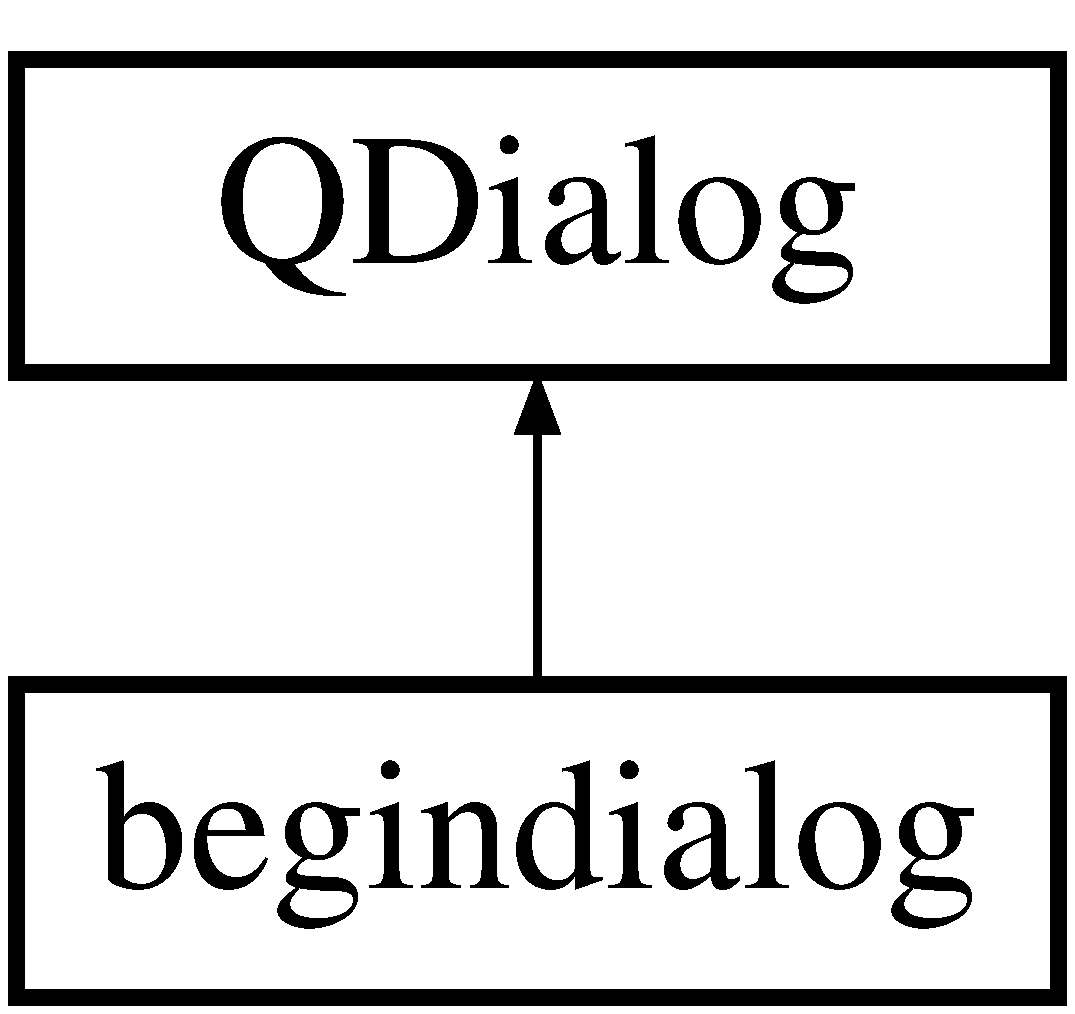
\includegraphics[height=2.000000cm]{classbegindialog}
\end{center}
\end{figure}
\subsection*{Public Member Functions}
\begin{DoxyCompactItemize}
\item 
\hyperlink{classbegindialog_a76bb9418e0b00fbb94c2cef459a83b08}{begindialog} (Q\-Widget $\ast$parent=0)
\begin{DoxyCompactList}\small\item\em Constructor for the class. \end{DoxyCompactList}\item 
\hyperlink{classbegindialog_a83236454b5fab5d4fee1ef0c6f0307eb}{$\sim$begindialog} ()
\item 
std\-::vector$<$ std\-::string $>$ \hyperlink{classbegindialog_a3614bf1959c37603e094d39640190123}{get\-Playernames} ()
\begin{DoxyCompactList}\small\item\em get\-Playernames Returns players names. \end{DoxyCompactList}\item 
\hyperlink{namespaceCourse_ab9a46ed9cd00485e318e5731ea2f78d9}{Course\-::\-Resource\-Map} \hyperlink{classbegindialog_a1fdc4bd90ddc27df8064bea149b14fbf}{get\-Starting\-Resources} ()
\begin{DoxyCompactList}\small\item\em get\-Starting\-Resources Returns amount of starting resources. \end{DoxyCompactList}\item 
int \hyperlink{classbegindialog_a0a0d98c8c33dc11b35293a9d6104e2d6}{get\-Resources\-To\-Win} ()
\begin{DoxyCompactList}\small\item\em get\-Resources\-To\-Win Returns amount of resources needed for a win. \end{DoxyCompactList}\end{DoxyCompactItemize}
\subsection*{Private Attributes}
\begin{DoxyCompactItemize}
\item 
Ui\-::begindialog $\ast$ \hyperlink{classbegindialog_a055ab69448a9247db34df24a4c0abddc}{ui}
\end{DoxyCompactItemize}


\subsection{Detailed Description}
The begindialog class shows pop-\/up window in the beginning of the game. Asks \par
for player names, amount of starting resources and amount of resources to win. 

\subsection{Constructor \& Destructor Documentation}
\hypertarget{classbegindialog_a76bb9418e0b00fbb94c2cef459a83b08}{\index{begindialog@{begindialog}!begindialog@{begindialog}}
\index{begindialog@{begindialog}!begindialog@{begindialog}}
\subsubsection[{begindialog}]{\setlength{\rightskip}{0pt plus 5cm}begindialog\-::begindialog (
\begin{DoxyParamCaption}
\item[{Q\-Widget $\ast$}]{parent = {\ttfamily 0}}
\end{DoxyParamCaption}
)\hspace{0.3cm}{\ttfamily [explicit]}}}\label{classbegindialog_a76bb9418e0b00fbb94c2cef459a83b08}


Constructor for the class. 


\begin{DoxyParams}{Parameters}
{\em parent} & can be used to point to a parent widget. Not used. \\
\hline
\end{DoxyParams}
\hypertarget{classbegindialog_a83236454b5fab5d4fee1ef0c6f0307eb}{\index{begindialog@{begindialog}!$\sim$begindialog@{$\sim$begindialog}}
\index{$\sim$begindialog@{$\sim$begindialog}!begindialog@{begindialog}}
\subsubsection[{$\sim$begindialog}]{\setlength{\rightskip}{0pt plus 5cm}begindialog\-::$\sim$begindialog (
\begin{DoxyParamCaption}
{}
\end{DoxyParamCaption}
)}}\label{classbegindialog_a83236454b5fab5d4fee1ef0c6f0307eb}


\subsection{Member Function Documentation}
\hypertarget{classbegindialog_a3614bf1959c37603e094d39640190123}{\index{begindialog@{begindialog}!get\-Playernames@{get\-Playernames}}
\index{get\-Playernames@{get\-Playernames}!begindialog@{begindialog}}
\subsubsection[{get\-Playernames}]{\setlength{\rightskip}{0pt plus 5cm}std\-::vector$<$ std\-::string $>$ begindialog\-::get\-Playernames (
\begin{DoxyParamCaption}
{}
\end{DoxyParamCaption}
)}}\label{classbegindialog_a3614bf1959c37603e094d39640190123}


get\-Playernames Returns players names. 

\begin{DoxyReturn}{Returns}
Vector of containing both player names. 
\end{DoxyReturn}
\hypertarget{classbegindialog_a0a0d98c8c33dc11b35293a9d6104e2d6}{\index{begindialog@{begindialog}!get\-Resources\-To\-Win@{get\-Resources\-To\-Win}}
\index{get\-Resources\-To\-Win@{get\-Resources\-To\-Win}!begindialog@{begindialog}}
\subsubsection[{get\-Resources\-To\-Win}]{\setlength{\rightskip}{0pt plus 5cm}int begindialog\-::get\-Resources\-To\-Win (
\begin{DoxyParamCaption}
{}
\end{DoxyParamCaption}
)}}\label{classbegindialog_a0a0d98c8c33dc11b35293a9d6104e2d6}


get\-Resources\-To\-Win Returns amount of resources needed for a win. 

\begin{DoxyReturn}{Returns}
Amount of resources needed for a win. 
\end{DoxyReturn}
\hypertarget{classbegindialog_a1fdc4bd90ddc27df8064bea149b14fbf}{\index{begindialog@{begindialog}!get\-Starting\-Resources@{get\-Starting\-Resources}}
\index{get\-Starting\-Resources@{get\-Starting\-Resources}!begindialog@{begindialog}}
\subsubsection[{get\-Starting\-Resources}]{\setlength{\rightskip}{0pt plus 5cm}{\bf Course\-::\-Resource\-Map} begindialog\-::get\-Starting\-Resources (
\begin{DoxyParamCaption}
{}
\end{DoxyParamCaption}
)}}\label{classbegindialog_a1fdc4bd90ddc27df8064bea149b14fbf}


get\-Starting\-Resources Returns amount of starting resources. 

\begin{DoxyReturn}{Returns}
Resource\-Map containing amounts of resources. 
\end{DoxyReturn}


\subsection{Member Data Documentation}
\hypertarget{classbegindialog_a055ab69448a9247db34df24a4c0abddc}{\index{begindialog@{begindialog}!ui@{ui}}
\index{ui@{ui}!begindialog@{begindialog}}
\subsubsection[{ui}]{\setlength{\rightskip}{0pt plus 5cm}Ui\-::begindialog$\ast$ begindialog\-::ui\hspace{0.3cm}{\ttfamily [private]}}}\label{classbegindialog_a055ab69448a9247db34df24a4c0abddc}


The documentation for this class was generated from the following files\-:\begin{DoxyCompactItemize}
\item 
Game/ui/\hyperlink{begindialog_8hh}{begindialog.\-hh}\item 
Game/ui/\hyperlink{begindialog_8cpp}{begindialog.\-cpp}\end{DoxyCompactItemize}

\hypertarget{classenddialog}{\section{enddialog Class Reference}
\label{classenddialog}\index{enddialog@{enddialog}}
}


The enddialog class shows pop-\/up window announcing the result when game ends.  




{\ttfamily \#include $<$enddialog.\-hh$>$}

Inheritance diagram for enddialog\-:\begin{figure}[H]
\begin{center}
\leavevmode
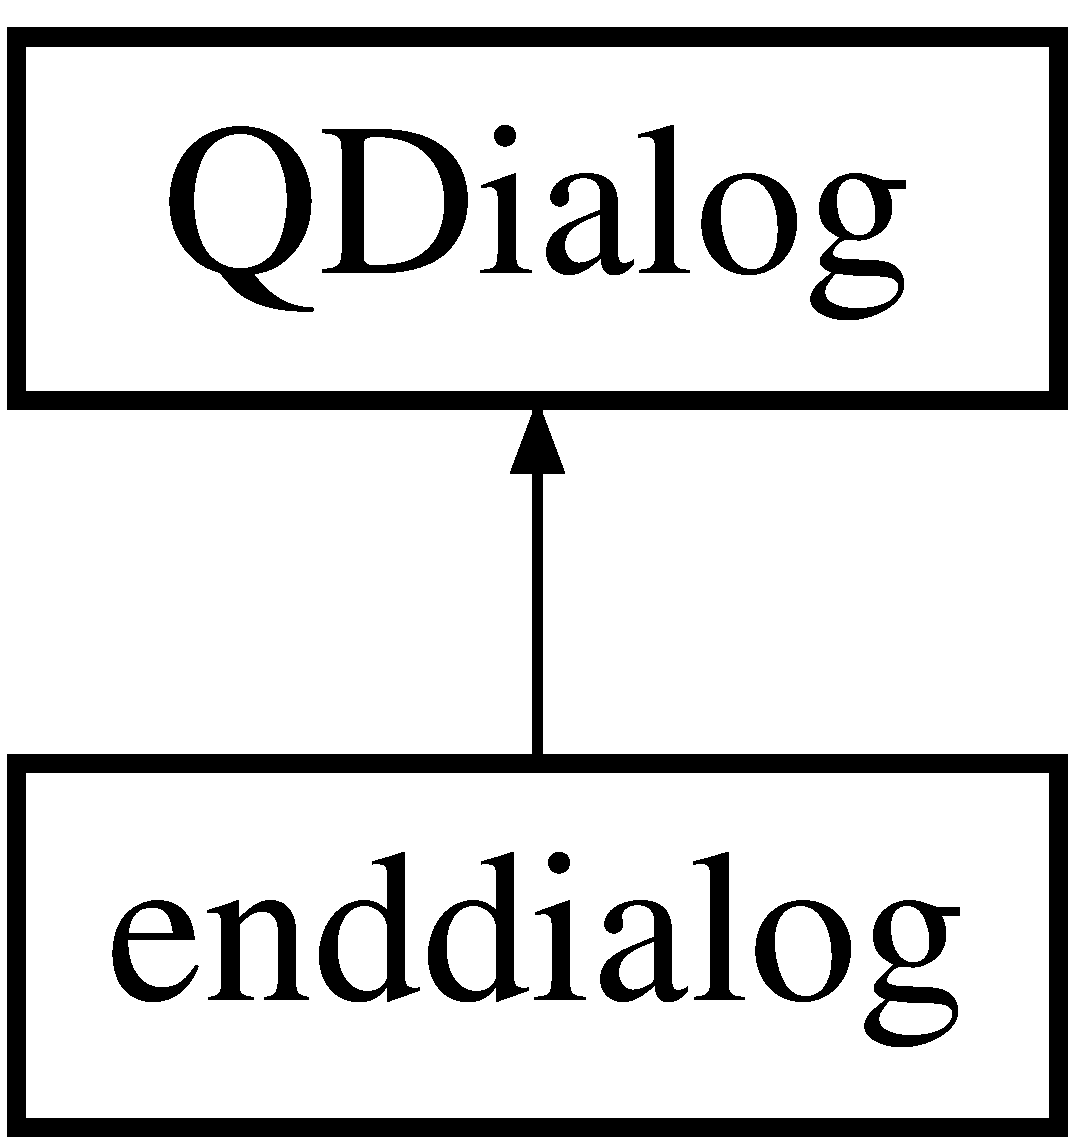
\includegraphics[height=2.000000cm]{classenddialog}
\end{center}
\end{figure}
\subsection*{Public Member Functions}
\begin{DoxyCompactItemize}
\item 
\hyperlink{classenddialog_a5dcbc64678b43043e16f74bd4c4dffb0}{enddialog} (Q\-Widget $\ast$parent=0)
\begin{DoxyCompactList}\small\item\em Constructor for the class. \end{DoxyCompactList}\item 
void \hyperlink{classenddialog_ab3da4bfad75f08deb94a5139799fcbb9}{set\-Winner} (std\-::vector$<$ std\-::shared\-\_\-ptr$<$ \hyperlink{classPlayer}{Player} $>$ $>$ winners, int round)
\begin{DoxyCompactList}\small\item\em set\-Winner Announces winner or a draw in the end of the game. \end{DoxyCompactList}\end{DoxyCompactItemize}


\subsection{Detailed Description}
The enddialog class shows pop-\/up window announcing the result when game ends. 

Has text label for game result and exit button for quitting the game. 

\subsection{Constructor \& Destructor Documentation}
\hypertarget{classenddialog_a5dcbc64678b43043e16f74bd4c4dffb0}{\index{enddialog@{enddialog}!enddialog@{enddialog}}
\index{enddialog@{enddialog}!enddialog@{enddialog}}
\subsubsection[{enddialog}]{\setlength{\rightskip}{0pt plus 5cm}enddialog\-::enddialog (
\begin{DoxyParamCaption}
\item[{Q\-Widget $\ast$}]{parent = {\ttfamily 0}}
\end{DoxyParamCaption}
)\hspace{0.3cm}{\ttfamily [explicit]}}}\label{classenddialog_a5dcbc64678b43043e16f74bd4c4dffb0}


Constructor for the class. 


\begin{DoxyParams}{Parameters}
{\em parent} & can be used to point to a parent widget. Not used. \\
\hline
\end{DoxyParams}


\subsection{Member Function Documentation}
\hypertarget{classenddialog_ab3da4bfad75f08deb94a5139799fcbb9}{\index{enddialog@{enddialog}!set\-Winner@{set\-Winner}}
\index{set\-Winner@{set\-Winner}!enddialog@{enddialog}}
\subsubsection[{set\-Winner}]{\setlength{\rightskip}{0pt plus 5cm}void enddialog\-::set\-Winner (
\begin{DoxyParamCaption}
\item[{std\-::vector$<$ std\-::shared\-\_\-ptr$<$ {\bf Player} $>$ $>$}]{winners, }
\item[{int}]{round}
\end{DoxyParamCaption}
)}}\label{classenddialog_ab3da4bfad75f08deb94a5139799fcbb9}


set\-Winner Announces winner or a draw in the end of the game. 


\begin{DoxyParams}{Parameters}
{\em winners} & Pointer to vector which has winner or winners. \\
\hline
{\em round} & Number of rounds played. \\
\hline
\end{DoxyParams}


The documentation for this class was generated from the following files\-:\begin{DoxyCompactItemize}
\item 
enddialog.\-hh\item 
enddialog.\-cpp\end{DoxyCompactItemize}

\hypertarget{classGameEventHandler}{\section{Game\-Event\-Handler Class Reference}
\label{classGameEventHandler}\index{Game\-Event\-Handler@{Game\-Event\-Handler}}
}


The \hyperlink{classGameEventHandler}{Game\-Event\-Handler} class controls and stores the game's status.  




{\ttfamily \#include $<$gameeventhandler.\-h$>$}

Inheritance diagram for Game\-Event\-Handler\-:\begin{figure}[H]
\begin{center}
\leavevmode
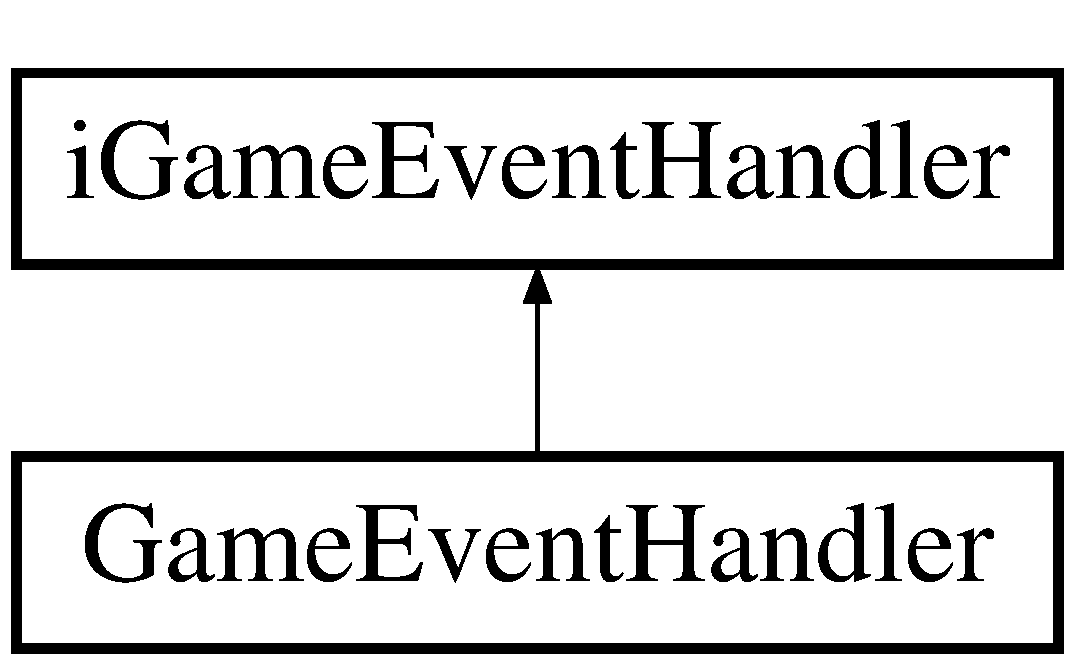
\includegraphics[height=2.000000cm]{classGameEventHandler}
\end{center}
\end{figure}
\subsection*{Public Member Functions}
\begin{DoxyCompactItemize}
\item 
\hypertarget{classGameEventHandler_a5c739015e6a26976d4941581c7f4852f}{\hyperlink{classGameEventHandler_a5c739015e6a26976d4941581c7f4852f}{Game\-Event\-Handler} ()}\label{classGameEventHandler_a5c739015e6a26976d4941581c7f4852f}

\begin{DoxyCompactList}\small\item\em Constructor for the class. \end{DoxyCompactList}\item 
bool \hyperlink{classGameEventHandler_a7b0209a6043ba6626228c5340e9a7892}{modify\-Resource} (std\-::shared\-\_\-ptr$<$ Course\-::\-Player\-Base $>$ player, Course\-::\-Basic\-Resource resource, int amount)
\begin{DoxyCompactList}\small\item\em Modify \hyperlink{classPlayer}{Player}'s resource. Can be used to both sum or subtract. \end{DoxyCompactList}\item 
bool \hyperlink{classGameEventHandler_acae1377e4a362a488b67bb7c8767a94e}{modify\-Resources} (std\-::shared\-\_\-ptr$<$ Course\-::\-Player\-Base $>$ player, Course\-::\-Resource\-Map resources)
\begin{DoxyCompactList}\small\item\em Modify \hyperlink{classPlayer}{Player}'s resources. Can be used to both sum or subtract. \end{DoxyCompactList}\item 
std\-::shared\-\_\-ptr$<$ \hyperlink{classPlayer}{Player} $>$ \hyperlink{classGameEventHandler_abdea4b1e077b65b05451a9a8fe679831}{get\-Player\-In\-Turn} ()
\begin{DoxyCompactList}\small\item\em Gets the player in turn. \end{DoxyCompactList}\item 
void \hyperlink{classGameEventHandler_ab103e178471df2a5c6f5f769bd1e0459}{set\-Player\-In\-Turn} (const std\-::shared\-\_\-ptr$<$ \hyperlink{classPlayer}{Player} $>$ player)
\begin{DoxyCompactList}\small\item\em Sets the player in turn. \end{DoxyCompactList}\item 
std\-::vector$<$ std\-::shared\-\_\-ptr\\*
$<$ \hyperlink{classPlayer}{Player} $>$ $>$ \hyperlink{classGameEventHandler_aa5ad66ca2e396c97ad2f9328234cacd9}{check\-Win\-Condition} (std\-::vector$<$ std\-::shared\-\_\-ptr$<$ \hyperlink{classPlayer}{Player} $>$$>$ players)
\begin{DoxyCompactList}\small\item\em Checks if players have won. \end{DoxyCompactList}\item 
void \hyperlink{classGameEventHandler_a1c5d965a153cf81b0d594cf49625a4d9}{set\-Resources\-To\-Win} (const int resources\-To\-Win)
\begin{DoxyCompactList}\small\item\em Sets the sum of resources needed to win the game. \end{DoxyCompactList}\item 
void \hyperlink{classGameEventHandler_a23bc60e5d802eb151d0f227c3ec75d82}{set\-Buying\-Flag} (const bool buying)
\begin{DoxyCompactList}\small\item\em Sets the flag telling that we are in the middle of buying something. \end{DoxyCompactList}\item 
bool \hyperlink{classGameEventHandler_a682951eb61bb9653a1a84bd72ee8ea9f}{is\-Player\-Buying} () const 
\begin{DoxyCompactList}\small\item\em Checks if we are in the middle of buying something. \end{DoxyCompactList}\item 
int \hyperlink{classGameEventHandler_a8d8ce2069c3bc1e96ca8d6bbfca6786a}{get\-Rounds} () const 
\begin{DoxyCompactList}\small\item\em Gets the amount of rounds the game has been played. \end{DoxyCompactList}\item 
int \hyperlink{classGameEventHandler_a8ab76d633c0cc009e47639171df7b0bd}{increase\-Rounds} ()
\begin{DoxyCompactList}\small\item\em Increases the game round by one. \end{DoxyCompactList}\end{DoxyCompactItemize}


\subsection{Detailed Description}
The \hyperlink{classGameEventHandler}{Game\-Event\-Handler} class controls and stores the game's status. 

Only one of these should exists at any given point in the time 

\subsection{Member Function Documentation}
\hypertarget{classGameEventHandler_aa5ad66ca2e396c97ad2f9328234cacd9}{\index{Game\-Event\-Handler@{Game\-Event\-Handler}!check\-Win\-Condition@{check\-Win\-Condition}}
\index{check\-Win\-Condition@{check\-Win\-Condition}!GameEventHandler@{Game\-Event\-Handler}}
\subsubsection[{check\-Win\-Condition}]{\setlength{\rightskip}{0pt plus 5cm}std\-::vector$<$ std\-::shared\-\_\-ptr$<$ {\bf Player} $>$ $>$ Game\-Event\-Handler\-::check\-Win\-Condition (
\begin{DoxyParamCaption}
\item[{std\-::vector$<$ std\-::shared\-\_\-ptr$<$ {\bf Player} $>$$>$}]{players}
\end{DoxyParamCaption}
)}}\label{classGameEventHandler_aa5ad66ca2e396c97ad2f9328234cacd9}


Checks if players have won. 


\begin{DoxyParams}{Parameters}
{\em players} & Vector of pointers to \hyperlink{classPlayer}{Player} objects. \\
\hline
\end{DoxyParams}
\begin{DoxyReturn}{Returns}
Vector of pointers to \hyperlink{classPlayer}{Player} objects that have won 
\end{DoxyReturn}
\hypertarget{classGameEventHandler_abdea4b1e077b65b05451a9a8fe679831}{\index{Game\-Event\-Handler@{Game\-Event\-Handler}!get\-Player\-In\-Turn@{get\-Player\-In\-Turn}}
\index{get\-Player\-In\-Turn@{get\-Player\-In\-Turn}!GameEventHandler@{Game\-Event\-Handler}}
\subsubsection[{get\-Player\-In\-Turn}]{\setlength{\rightskip}{0pt plus 5cm}std\-::shared\-\_\-ptr$<$ {\bf Player} $>$ Game\-Event\-Handler\-::get\-Player\-In\-Turn (
\begin{DoxyParamCaption}
{}
\end{DoxyParamCaption}
)}}\label{classGameEventHandler_abdea4b1e077b65b05451a9a8fe679831}


Gets the player in turn. 

\begin{DoxyReturn}{Returns}
the player whose turn it is currently 
\end{DoxyReturn}
\hypertarget{classGameEventHandler_a8d8ce2069c3bc1e96ca8d6bbfca6786a}{\index{Game\-Event\-Handler@{Game\-Event\-Handler}!get\-Rounds@{get\-Rounds}}
\index{get\-Rounds@{get\-Rounds}!GameEventHandler@{Game\-Event\-Handler}}
\subsubsection[{get\-Rounds}]{\setlength{\rightskip}{0pt plus 5cm}int Game\-Event\-Handler\-::get\-Rounds (
\begin{DoxyParamCaption}
{}
\end{DoxyParamCaption}
) const}}\label{classGameEventHandler_a8d8ce2069c3bc1e96ca8d6bbfca6786a}


Gets the amount of rounds the game has been played. 

\begin{DoxyReturn}{Returns}
Amount of rounds 
\end{DoxyReturn}
\hypertarget{classGameEventHandler_a8ab76d633c0cc009e47639171df7b0bd}{\index{Game\-Event\-Handler@{Game\-Event\-Handler}!increase\-Rounds@{increase\-Rounds}}
\index{increase\-Rounds@{increase\-Rounds}!GameEventHandler@{Game\-Event\-Handler}}
\subsubsection[{increase\-Rounds}]{\setlength{\rightskip}{0pt plus 5cm}int Game\-Event\-Handler\-::increase\-Rounds (
\begin{DoxyParamCaption}
{}
\end{DoxyParamCaption}
)}}\label{classGameEventHandler_a8ab76d633c0cc009e47639171df7b0bd}


Increases the game round by one. 

\begin{DoxyReturn}{Returns}
Amount of rounds after the increase 
\end{DoxyReturn}
\hypertarget{classGameEventHandler_a682951eb61bb9653a1a84bd72ee8ea9f}{\index{Game\-Event\-Handler@{Game\-Event\-Handler}!is\-Player\-Buying@{is\-Player\-Buying}}
\index{is\-Player\-Buying@{is\-Player\-Buying}!GameEventHandler@{Game\-Event\-Handler}}
\subsubsection[{is\-Player\-Buying}]{\setlength{\rightskip}{0pt plus 5cm}bool Game\-Event\-Handler\-::is\-Player\-Buying (
\begin{DoxyParamCaption}
{}
\end{DoxyParamCaption}
) const}}\label{classGameEventHandler_a682951eb61bb9653a1a84bd72ee8ea9f}


Checks if we are in the middle of buying something. 

\begin{DoxyReturn}{Returns}
Boolean value telling if we are buying something 
\end{DoxyReturn}
\hypertarget{classGameEventHandler_a7b0209a6043ba6626228c5340e9a7892}{\index{Game\-Event\-Handler@{Game\-Event\-Handler}!modify\-Resource@{modify\-Resource}}
\index{modify\-Resource@{modify\-Resource}!GameEventHandler@{Game\-Event\-Handler}}
\subsubsection[{modify\-Resource}]{\setlength{\rightskip}{0pt plus 5cm}bool Game\-Event\-Handler\-::modify\-Resource (
\begin{DoxyParamCaption}
\item[{std\-::shared\-\_\-ptr$<$ Course\-::\-Player\-Base $>$}]{player, }
\item[{Course\-::\-Basic\-Resource}]{resource, }
\item[{int}]{amount}
\end{DoxyParamCaption}
)}}\label{classGameEventHandler_a7b0209a6043ba6626228c5340e9a7892}


Modify \hyperlink{classPlayer}{Player}'s resource. Can be used to both sum or subtract. 


\begin{DoxyParams}{Parameters}
{\em player} & Pointer to the \hyperlink{classPlayer}{Player} whose resource is being modified. \\
\hline
{\em resource} & Defines the modified resource. \\
\hline
{\em amount} & Defines the amount of change. \\
\hline
\end{DoxyParams}
\begin{DoxyPostcond}{Postcondition}
Exception guarantee\-: Basic 
\end{DoxyPostcond}
\begin{DoxyReturn}{Returns}
True -\/ Modification was succesful. \par
False -\/ Modification failed. \par

\end{DoxyReturn}
\hypertarget{classGameEventHandler_acae1377e4a362a488b67bb7c8767a94e}{\index{Game\-Event\-Handler@{Game\-Event\-Handler}!modify\-Resources@{modify\-Resources}}
\index{modify\-Resources@{modify\-Resources}!GameEventHandler@{Game\-Event\-Handler}}
\subsubsection[{modify\-Resources}]{\setlength{\rightskip}{0pt plus 5cm}bool Game\-Event\-Handler\-::modify\-Resources (
\begin{DoxyParamCaption}
\item[{std\-::shared\-\_\-ptr$<$ Course\-::\-Player\-Base $>$}]{player, }
\item[{Course\-::\-Resource\-Map}]{resources}
\end{DoxyParamCaption}
)}}\label{classGameEventHandler_acae1377e4a362a488b67bb7c8767a94e}


Modify \hyperlink{classPlayer}{Player}'s resources. Can be used to both sum or subtract. 


\begin{DoxyParams}{Parameters}
{\em player} & Pointer to the \hyperlink{classPlayer}{Player} whose resources are being modified. \\
\hline
{\em resources} & Resource\-Map containing change amounts. \\
\hline
\end{DoxyParams}
\begin{DoxyReturn}{Returns}
True -\/ Modification was succesful. \par
False -\/ Modification failed. \par

\end{DoxyReturn}
\hypertarget{classGameEventHandler_a23bc60e5d802eb151d0f227c3ec75d82}{\index{Game\-Event\-Handler@{Game\-Event\-Handler}!set\-Buying\-Flag@{set\-Buying\-Flag}}
\index{set\-Buying\-Flag@{set\-Buying\-Flag}!GameEventHandler@{Game\-Event\-Handler}}
\subsubsection[{set\-Buying\-Flag}]{\setlength{\rightskip}{0pt plus 5cm}void Game\-Event\-Handler\-::set\-Buying\-Flag (
\begin{DoxyParamCaption}
\item[{const bool}]{buying}
\end{DoxyParamCaption}
)}}\label{classGameEventHandler_a23bc60e5d802eb151d0f227c3ec75d82}


Sets the flag telling that we are in the middle of buying something. 


\begin{DoxyParams}{Parameters}
{\em buying} & Flag for buying \\
\hline
\end{DoxyParams}
\hypertarget{classGameEventHandler_ab103e178471df2a5c6f5f769bd1e0459}{\index{Game\-Event\-Handler@{Game\-Event\-Handler}!set\-Player\-In\-Turn@{set\-Player\-In\-Turn}}
\index{set\-Player\-In\-Turn@{set\-Player\-In\-Turn}!GameEventHandler@{Game\-Event\-Handler}}
\subsubsection[{set\-Player\-In\-Turn}]{\setlength{\rightskip}{0pt plus 5cm}void Game\-Event\-Handler\-::set\-Player\-In\-Turn (
\begin{DoxyParamCaption}
\item[{const std\-::shared\-\_\-ptr$<$ {\bf Player} $>$}]{player}
\end{DoxyParamCaption}
)}}\label{classGameEventHandler_ab103e178471df2a5c6f5f769bd1e0459}


Sets the player in turn. 


\begin{DoxyParams}{Parameters}
{\em player} & Pointer to the \hyperlink{classPlayer}{Player}. \\
\hline
\end{DoxyParams}
\hypertarget{classGameEventHandler_a1c5d965a153cf81b0d594cf49625a4d9}{\index{Game\-Event\-Handler@{Game\-Event\-Handler}!set\-Resources\-To\-Win@{set\-Resources\-To\-Win}}
\index{set\-Resources\-To\-Win@{set\-Resources\-To\-Win}!GameEventHandler@{Game\-Event\-Handler}}
\subsubsection[{set\-Resources\-To\-Win}]{\setlength{\rightskip}{0pt plus 5cm}void Game\-Event\-Handler\-::set\-Resources\-To\-Win (
\begin{DoxyParamCaption}
\item[{const int}]{resources\-To\-Win}
\end{DoxyParamCaption}
)}}\label{classGameEventHandler_a1c5d965a153cf81b0d594cf49625a4d9}


Sets the sum of resources needed to win the game. 


\begin{DoxyParams}{Parameters}
{\em resources\-To\-Win} & Amount of resources as a sum \\
\hline
\end{DoxyParams}


The documentation for this class was generated from the following files\-:\begin{DoxyCompactItemize}
\item 
gameeventhandler.\-h\item 
gameeventhandler.\-cpp\end{DoxyCompactItemize}

\hypertarget{classMapWindow}{\section{Map\-Window Class Reference}
\label{classMapWindow}\index{Map\-Window@{Map\-Window}}
}


The \hyperlink{classMapWindow}{Map\-Window} class is the main game window.  




{\ttfamily \#include $<$mapwindow.\-hh$>$}

Inheritance diagram for Map\-Window\-:\begin{figure}[H]
\begin{center}
\leavevmode
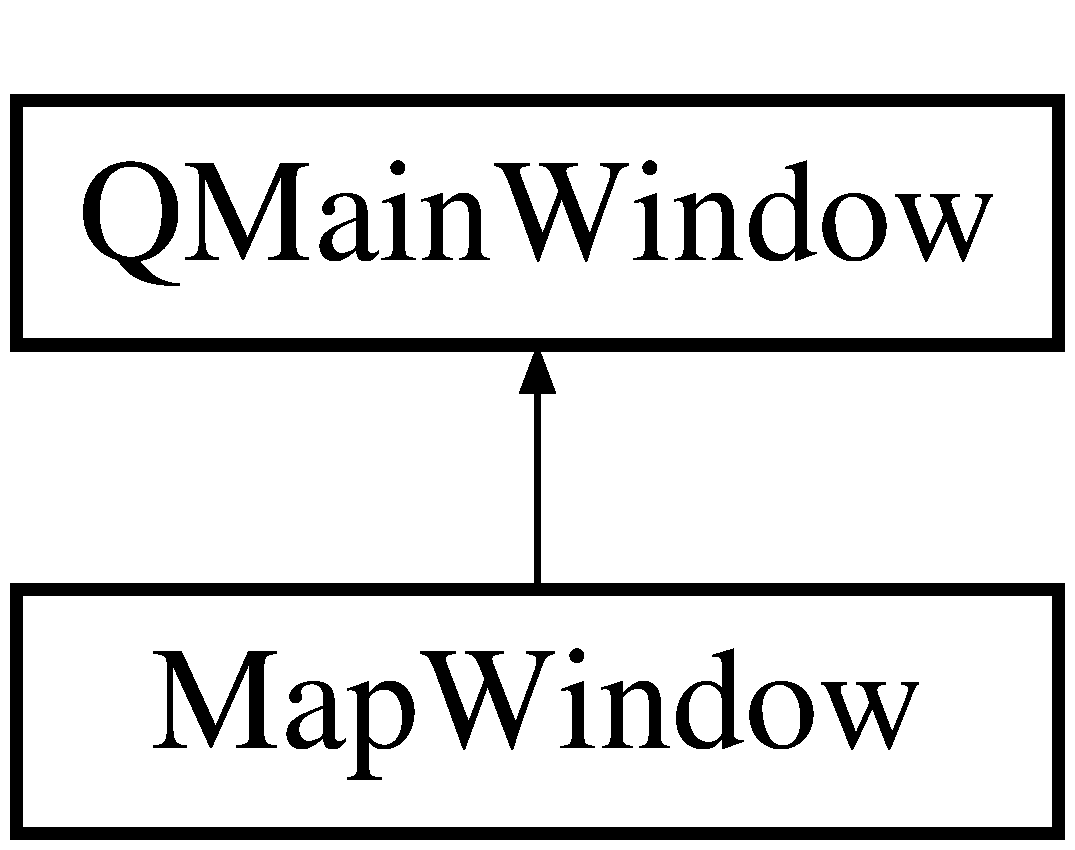
\includegraphics[height=2.000000cm]{classMapWindow}
\end{center}
\end{figure}
\subsection*{Public Slots}
\begin{DoxyCompactItemize}
\item 
void \hyperlink{classMapWindow_a39948451de86944d283ac9fc972cf271}{place\-Object} (Course\-::\-Object\-Id tile\-I\-D)
\begin{DoxyCompactList}\small\item\em Sets a Placeable\-Game\-Object onto a tile and sets \par
owners for required objects. \end{DoxyCompactList}\item 
bool \hyperlink{classMapWindow_a014ed30c996e95f034a71e3ab66947ef}{event\-Filter} (Q\-Object $\ast$watched, Q\-Event $\ast$event)
\begin{DoxyCompactList}\small\item\em Shows and hides info text of building and hiring buttons when \par
 hovered over with mouse. \end{DoxyCompactList}\end{DoxyCompactItemize}
\subsection*{Public Member Functions}
\begin{DoxyCompactItemize}
\item 
\hyperlink{classMapWindow_a1384c7a04267c23e413304b575870ddf}{Map\-Window} (Q\-Widget $\ast$parent=0, std\-::shared\-\_\-ptr$<$ \hyperlink{classGameEventHandler}{Game\-Event\-Handler} $>$ G\-E\-Handler=\{\}, std\-::shared\-\_\-ptr$<$ \hyperlink{classObjectManager}{Object\-Manager} $>$ obj\-Man=\{\})
\begin{DoxyCompactList}\small\item\em Constructor for the class. \end{DoxyCompactList}\item 
\hypertarget{classMapWindow_a12edf2fb9ac7a6ebf501c0da8aa327dc}{\hyperlink{classMapWindow_a12edf2fb9ac7a6ebf501c0da8aa327dc}{$\sim$\-Map\-Window} ()}\label{classMapWindow_a12edf2fb9ac7a6ebf501c0da8aa327dc}

\begin{DoxyCompactList}\small\item\em Constructor for the class. \end{DoxyCompactList}\item 
std\-::shared\-\_\-ptr$<$ \hyperlink{classGameEventHandler}{Game\-Event\-Handler} $>$ \hyperlink{classMapWindow_a1ec4c2876b71f131fa00f1189e2c9a99}{get\-G\-E\-Handler} ()
\begin{DoxyCompactList}\small\item\em Gets a pointer to the \hyperlink{classGameEventHandler}{Game\-Event\-Handler}. \end{DoxyCompactList}\item 
std\-::shared\-\_\-ptr$<$ \hyperlink{classObjectManager}{Object\-Manager} $>$ \hyperlink{classMapWindow_a5e172f1f313d7390306515cdb0fc3305}{get\-Obj\-Man} ()
\begin{DoxyCompactList}\small\item\em Gets a pointer to the \hyperlink{classObjectManager}{Object\-Manager}. \end{DoxyCompactList}\item 
void \hyperlink{classMapWindow_a7b5fcf2d1ba7c211faabdfd3c81cc5b5}{set\-Size} (int width, int height)
\begin{DoxyCompactList}\small\item\em Sets the game map. \end{DoxyCompactList}\item 
void \hyperlink{classMapWindow_a9d5c988b6ac8dced6aa128df160be6cc}{set\-Scale} (int scale)
\begin{DoxyCompactList}\small\item\em Sets the game map tile scale. \end{DoxyCompactList}\item 
\hypertarget{classMapWindow_a9eebe13b89eacd419ed5c250a9fc1d2e}{void \hyperlink{classMapWindow_a9eebe13b89eacd419ed5c250a9fc1d2e}{resize} ()}\label{classMapWindow_a9eebe13b89eacd419ed5c250a9fc1d2e}

\begin{DoxyCompactList}\small\item\em Recreates the game map base according to the saved dimensions. \end{DoxyCompactList}\item 
void \hyperlink{classMapWindow_a84951fe90f52cd94b73fdc7b0a4e4899}{draw\-Item} (std\-::shared\-\_\-ptr$<$ Course\-::\-Game\-Object $>$ obj, int offset=0)
\begin{DoxyCompactList}\small\item\em Draws a Game\-Object on the game map. \end{DoxyCompactList}\item 
void \hyperlink{classMapWindow_a88384cf195d4cec6e4779d2f6b83b675}{remove\-Item} (std\-::shared\-\_\-ptr$<$ Course\-::\-Game\-Object $>$ obj)
\begin{DoxyCompactList}\small\item\em Remove a Game\-Object from the game map. \end{DoxyCompactList}\item 
void \hyperlink{classMapWindow_a40b4e18c08d80bafcf006fafe16d75c2}{update\-Item} (std\-::shared\-\_\-ptr$<$ Course\-::\-Game\-Object $>$ obj)
\begin{DoxyCompactList}\small\item\em Updates a Game\-Object on the game map. \end{DoxyCompactList}\item 
void \hyperlink{classMapWindow_ab834c94bbb2a4e209eda3c7f283e2cd2}{change\-Turn} (const std\-::shared\-\_\-ptr$<$ \hyperlink{classPlayer}{Player} $>$ player)
\begin{DoxyCompactList}\small\item\em Changes the U\-I for the next player in turn. \end{DoxyCompactList}\item 
void \hyperlink{classMapWindow_aa0ab33facccac2bdfafcc68468725f55}{setup\-U\-I} (int resources\-To\-Win)
\begin{DoxyCompactList}\small\item\em Sets up certain fixed elements in the U\-I when a game is started. \end{DoxyCompactList}\end{DoxyCompactItemize}


\subsection{Detailed Description}
The \hyperlink{classMapWindow}{Map\-Window} class is the main game window. 

The U\-I consists of the game map, buttons for buying objects and \par
information related to the game state. 

\subsection{Constructor \& Destructor Documentation}
\hypertarget{classMapWindow_a1384c7a04267c23e413304b575870ddf}{\index{Map\-Window@{Map\-Window}!Map\-Window@{Map\-Window}}
\index{Map\-Window@{Map\-Window}!MapWindow@{Map\-Window}}
\subsubsection[{Map\-Window}]{\setlength{\rightskip}{0pt plus 5cm}Map\-Window\-::\-Map\-Window (
\begin{DoxyParamCaption}
\item[{Q\-Widget $\ast$}]{parent = {\ttfamily 0}, }
\item[{std\-::shared\-\_\-ptr$<$ {\bf Game\-Event\-Handler} $>$}]{G\-E\-Handler = {\ttfamily \{\}}, }
\item[{std\-::shared\-\_\-ptr$<$ {\bf Object\-Manager} $>$}]{obj\-Man = {\ttfamily \{\}}}
\end{DoxyParamCaption}
)\hspace{0.3cm}{\ttfamily [explicit]}}}\label{classMapWindow_a1384c7a04267c23e413304b575870ddf}


Constructor for the class. 


\begin{DoxyParams}{Parameters}
{\em parent} & can be used to point to a parent widget. Not used. \\
\hline
{\em G\-E\-Handler} & points to the \hyperlink{classGameEventHandler}{Game\-Event\-Handler} \\
\hline
{\em obj\-Man} & points to the \hyperlink{classObjectManager}{Object\-Manager} \\
\hline
\end{DoxyParams}


\subsection{Member Function Documentation}
\hypertarget{classMapWindow_ab834c94bbb2a4e209eda3c7f283e2cd2}{\index{Map\-Window@{Map\-Window}!change\-Turn@{change\-Turn}}
\index{change\-Turn@{change\-Turn}!MapWindow@{Map\-Window}}
\subsubsection[{change\-Turn}]{\setlength{\rightskip}{0pt plus 5cm}void Map\-Window\-::change\-Turn (
\begin{DoxyParamCaption}
\item[{const std\-::shared\-\_\-ptr$<$ {\bf Player} $>$}]{player}
\end{DoxyParamCaption}
)}}\label{classMapWindow_ab834c94bbb2a4e209eda3c7f283e2cd2}


Changes the U\-I for the next player in turn. 


\begin{DoxyParams}{Parameters}
{\em player} & pointer to a \hyperlink{classPlayer}{Player} object whose turn it's going to be \\
\hline
\end{DoxyParams}
\hypertarget{classMapWindow_a84951fe90f52cd94b73fdc7b0a4e4899}{\index{Map\-Window@{Map\-Window}!draw\-Item@{draw\-Item}}
\index{draw\-Item@{draw\-Item}!MapWindow@{Map\-Window}}
\subsubsection[{draw\-Item}]{\setlength{\rightskip}{0pt plus 5cm}void Map\-Window\-::draw\-Item (
\begin{DoxyParamCaption}
\item[{std\-::shared\-\_\-ptr$<$ Course\-::\-Game\-Object $>$}]{obj, }
\item[{int}]{offset = {\ttfamily 0}}
\end{DoxyParamCaption}
)}}\label{classMapWindow_a84951fe90f52cd94b73fdc7b0a4e4899}


Draws a Game\-Object on the game map. 


\begin{DoxyParams}{Parameters}
{\em obj} & object to be drawn \\
\hline
{\em offset} & of the object in coordinates \\
\hline
\end{DoxyParams}
\begin{DoxyNote}{Note}
Offset is used when drawing smaller object in different spots inside tiles. 
\end{DoxyNote}
\hypertarget{classMapWindow_a014ed30c996e95f034a71e3ab66947ef}{\index{Map\-Window@{Map\-Window}!event\-Filter@{event\-Filter}}
\index{event\-Filter@{event\-Filter}!MapWindow@{Map\-Window}}
\subsubsection[{event\-Filter}]{\setlength{\rightskip}{0pt plus 5cm}bool Map\-Window\-::event\-Filter (
\begin{DoxyParamCaption}
\item[{Q\-Object $\ast$}]{watched, }
\item[{Q\-Event $\ast$}]{event}
\end{DoxyParamCaption}
)\hspace{0.3cm}{\ttfamily [slot]}}}\label{classMapWindow_a014ed30c996e95f034a71e3ab66947ef}


Shows and hides info text of building and hiring buttons when \par
 hovered over with mouse. 


\begin{DoxyParams}{Parameters}
{\em watched} & Objects of buttons that are being tracked for mouse hovering. \\
\hline
{\em event} & Enter or leave events when mouse hovering over a button. \\
\hline
\end{DoxyParams}
\begin{DoxyReturn}{Returns}
Event to parent class 
\end{DoxyReturn}
\hypertarget{classMapWindow_a1ec4c2876b71f131fa00f1189e2c9a99}{\index{Map\-Window@{Map\-Window}!get\-G\-E\-Handler@{get\-G\-E\-Handler}}
\index{get\-G\-E\-Handler@{get\-G\-E\-Handler}!MapWindow@{Map\-Window}}
\subsubsection[{get\-G\-E\-Handler}]{\setlength{\rightskip}{0pt plus 5cm}std\-::shared\-\_\-ptr$<$ {\bf Game\-Event\-Handler} $>$ Map\-Window\-::get\-G\-E\-Handler (
\begin{DoxyParamCaption}
{}
\end{DoxyParamCaption}
)}}\label{classMapWindow_a1ec4c2876b71f131fa00f1189e2c9a99}


Gets a pointer to the \hyperlink{classGameEventHandler}{Game\-Event\-Handler}. 

\begin{DoxyReturn}{Returns}
Pointer to the \hyperlink{classGameEventHandler}{Game\-Event\-Handler} 
\end{DoxyReturn}
\hypertarget{classMapWindow_a5e172f1f313d7390306515cdb0fc3305}{\index{Map\-Window@{Map\-Window}!get\-Obj\-Man@{get\-Obj\-Man}}
\index{get\-Obj\-Man@{get\-Obj\-Man}!MapWindow@{Map\-Window}}
\subsubsection[{get\-Obj\-Man}]{\setlength{\rightskip}{0pt plus 5cm}std\-::shared\-\_\-ptr$<$ {\bf Object\-Manager} $>$ Map\-Window\-::get\-Obj\-Man (
\begin{DoxyParamCaption}
{}
\end{DoxyParamCaption}
)}}\label{classMapWindow_a5e172f1f313d7390306515cdb0fc3305}


Gets a pointer to the \hyperlink{classObjectManager}{Object\-Manager}. 

\begin{DoxyReturn}{Returns}
Pointer to the \hyperlink{classObjectManager}{Object\-Manager} 
\end{DoxyReturn}
\hypertarget{classMapWindow_a39948451de86944d283ac9fc972cf271}{\index{Map\-Window@{Map\-Window}!place\-Object@{place\-Object}}
\index{place\-Object@{place\-Object}!MapWindow@{Map\-Window}}
\subsubsection[{place\-Object}]{\setlength{\rightskip}{0pt plus 5cm}void Map\-Window\-::place\-Object (
\begin{DoxyParamCaption}
\item[{Course\-::\-Object\-Id}]{tile\-I\-D}
\end{DoxyParamCaption}
)\hspace{0.3cm}{\ttfamily [slot]}}}\label{classMapWindow_a39948451de86944d283ac9fc972cf271}


Sets a Placeable\-Game\-Object onto a tile and sets \par
owners for required objects. 


\begin{DoxyParams}{Parameters}
{\em tile\-I\-D} & of the tile clicked \\
\hline
\end{DoxyParams}
\begin{DoxyNote}{Note}
Executed when a tile is clicked on the map 
\end{DoxyNote}
\hypertarget{classMapWindow_a88384cf195d4cec6e4779d2f6b83b675}{\index{Map\-Window@{Map\-Window}!remove\-Item@{remove\-Item}}
\index{remove\-Item@{remove\-Item}!MapWindow@{Map\-Window}}
\subsubsection[{remove\-Item}]{\setlength{\rightskip}{0pt plus 5cm}void Map\-Window\-::remove\-Item (
\begin{DoxyParamCaption}
\item[{std\-::shared\-\_\-ptr$<$ Course\-::\-Game\-Object $>$}]{obj}
\end{DoxyParamCaption}
)}}\label{classMapWindow_a88384cf195d4cec6e4779d2f6b83b675}


Remove a Game\-Object from the game map. 


\begin{DoxyParams}{Parameters}
{\em obj} & object to be removed \\
\hline
\end{DoxyParams}
\hypertarget{classMapWindow_a9d5c988b6ac8dced6aa128df160be6cc}{\index{Map\-Window@{Map\-Window}!set\-Scale@{set\-Scale}}
\index{set\-Scale@{set\-Scale}!MapWindow@{Map\-Window}}
\subsubsection[{set\-Scale}]{\setlength{\rightskip}{0pt plus 5cm}void Map\-Window\-::set\-Scale (
\begin{DoxyParamCaption}
\item[{int}]{scale}
\end{DoxyParamCaption}
)}}\label{classMapWindow_a9d5c988b6ac8dced6aa128df160be6cc}


Sets the game map tile scale. 


\begin{DoxyParams}{Parameters}
{\em scale} & of the tiles \\
\hline
\end{DoxyParams}
\hypertarget{classMapWindow_a7b5fcf2d1ba7c211faabdfd3c81cc5b5}{\index{Map\-Window@{Map\-Window}!set\-Size@{set\-Size}}
\index{set\-Size@{set\-Size}!MapWindow@{Map\-Window}}
\subsubsection[{set\-Size}]{\setlength{\rightskip}{0pt plus 5cm}void Map\-Window\-::set\-Size (
\begin{DoxyParamCaption}
\item[{int}]{width, }
\item[{int}]{height}
\end{DoxyParamCaption}
)}}\label{classMapWindow_a7b5fcf2d1ba7c211faabdfd3c81cc5b5}


Sets the game map. 


\begin{DoxyParams}{Parameters}
{\em width} & of the map \\
\hline
{\em height} & of the map \\
\hline
\end{DoxyParams}
\hypertarget{classMapWindow_aa0ab33facccac2bdfafcc68468725f55}{\index{Map\-Window@{Map\-Window}!setup\-U\-I@{setup\-U\-I}}
\index{setup\-U\-I@{setup\-U\-I}!MapWindow@{Map\-Window}}
\subsubsection[{setup\-U\-I}]{\setlength{\rightskip}{0pt plus 5cm}void Map\-Window\-::setup\-U\-I (
\begin{DoxyParamCaption}
\item[{int}]{resources\-To\-Win}
\end{DoxyParamCaption}
)}}\label{classMapWindow_aa0ab33facccac2bdfafcc68468725f55}


Sets up certain fixed elements in the U\-I when a game is started. 


\begin{DoxyParams}{Parameters}
{\em resources\-To\-Win} & Amount of resources needed to win the game \\
\hline
\end{DoxyParams}
\hypertarget{classMapWindow_a40b4e18c08d80bafcf006fafe16d75c2}{\index{Map\-Window@{Map\-Window}!update\-Item@{update\-Item}}
\index{update\-Item@{update\-Item}!MapWindow@{Map\-Window}}
\subsubsection[{update\-Item}]{\setlength{\rightskip}{0pt plus 5cm}void Map\-Window\-::update\-Item (
\begin{DoxyParamCaption}
\item[{std\-::shared\-\_\-ptr$<$ Course\-::\-Game\-Object $>$}]{obj}
\end{DoxyParamCaption}
)}}\label{classMapWindow_a40b4e18c08d80bafcf006fafe16d75c2}


Updates a Game\-Object on the game map. 


\begin{DoxyParams}{Parameters}
{\em obj} & object to be updated \\
\hline
\end{DoxyParams}
\begin{DoxyNote}{Note}
The objects location, shape and color are all updated if needed. 
\end{DoxyNote}


The documentation for this class was generated from the following files\-:\begin{DoxyCompactItemize}
\item 
mapwindow.\-hh\item 
mapwindow.\-cc\end{DoxyCompactItemize}

\hypertarget{classObjectManager}{\section{Object\-Manager Class Reference}
\label{classObjectManager}\index{Object\-Manager@{Object\-Manager}}
}


The \hyperlink{classObjectManager}{Object\-Manager} class stores Players and Game\-Objects \par
(Tiles, Buildings and workers).  




{\ttfamily \#include $<$objectmanager.\-h$>$}

Inheritance diagram for Object\-Manager\-:\begin{figure}[H]
\begin{center}
\leavevmode
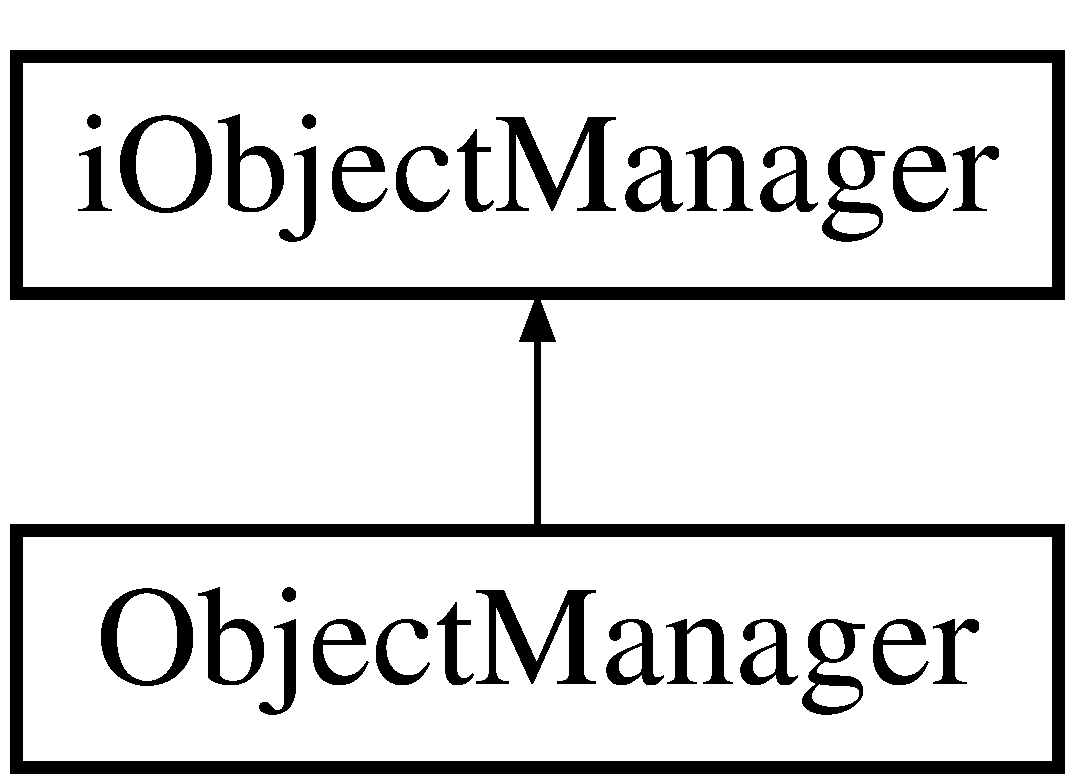
\includegraphics[height=2.000000cm]{classObjectManager}
\end{center}
\end{figure}
\subsection*{Public Member Functions}
\begin{DoxyCompactItemize}
\item 
\hypertarget{classObjectManager_a6fa9372c7c3a8da88412f4158ca3dfd9}{\hyperlink{classObjectManager_a6fa9372c7c3a8da88412f4158ca3dfd9}{Object\-Manager} ()}\label{classObjectManager_a6fa9372c7c3a8da88412f4158ca3dfd9}

\begin{DoxyCompactList}\small\item\em Constructor for the class. \end{DoxyCompactList}\item 
void \hyperlink{classObjectManager_a00b483db15dd68a6da5b6dd42a3cdfe0}{add\-Tiles} (const std\-::vector$<$ std\-::shared\-\_\-ptr$<$ Course\-::\-Tile\-Base $>$$>$ \&tiles)
\begin{DoxyCompactList}\small\item\em Adds new tiles to the \hyperlink{classObjectManager}{Object\-Manager}. \end{DoxyCompactList}\item 
std\-::shared\-\_\-ptr$<$ Course\-::\-Tile\-Base $>$ \hyperlink{classObjectManager_a5e9109ea92cf452ffdf02ed8cc6f8260}{get\-Tile} (const Course\-::\-Coordinate \&coordinate)
\begin{DoxyCompactList}\small\item\em Returns a shared pointer to a Tile that has specified coordinate. \end{DoxyCompactList}\item 
std\-::shared\-\_\-ptr$<$ Course\-::\-Tile\-Base $>$ \hyperlink{classObjectManager_a1bc804e3771e3a40bce0cc462ec35b97}{get\-Tile} (const Course\-::\-Object\-Id \&id)
\begin{DoxyCompactList}\small\item\em Returns a shared pointer to a Tile that has specified I\-D. \end{DoxyCompactList}\item 
std\-::vector$<$ std\-::shared\-\_\-ptr\\*
$<$ Course\-::\-Tile\-Base $>$ $>$ \hyperlink{classObjectManager_a891e222168b45f7cacb522852fb45cf1}{get\-Tiles} (const std\-::vector$<$ Course\-::\-Coordinate $>$ \&coordinates)
\begin{DoxyCompactList}\small\item\em Returns a vector of shared pointers to Tiles specified by a vector of Coordinates. \end{DoxyCompactList}\item 
const std\-::vector\\*
$<$ std\-::shared\-\_\-ptr\\*
$<$ Course\-::\-Tile\-Base $>$ $>$ \hyperlink{classObjectManager_adf0c963a866b9e22acb3c5f8af0a5f87}{get\-Tiles} () const 
\begin{DoxyCompactList}\small\item\em Returns a vector of shared pointers to all stored Tiles. \end{DoxyCompactList}\item 
void \hyperlink{classObjectManager_a87d894cca083ccc6f1e764f647627850}{add\-Player} (const std\-::shared\-\_\-ptr$<$ \hyperlink{classPlayer}{Player} $>$ player)
\begin{DoxyCompactList}\small\item\em Adds a new \hyperlink{classPlayer}{Player} to the \hyperlink{classObjectManager}{Object\-Manager}. \end{DoxyCompactList}\item 
const std\-::vector\\*
$<$ std\-::shared\-\_\-ptr$<$ \hyperlink{classPlayer}{Player} $>$ $>$ \hyperlink{classObjectManager_a192bf2fa88041eeb0ba8b35723b99504}{get\-Players} () const 
\begin{DoxyCompactList}\small\item\em Returns a vector of shared pointers to all stored Players. \end{DoxyCompactList}\item 
bool \hyperlink{classObjectManager_ac658e0043de7550745f723bc7035cd8d}{is\-Last\-Player} (const std\-::shared\-\_\-ptr$<$ \hyperlink{classPlayer}{Player} $>$ player)
\begin{DoxyCompactList}\small\item\em Returns whether a player is the last player to act. \end{DoxyCompactList}\item 
void \hyperlink{classObjectManager_a27ae17c7d302790f6727b29fdc523092}{add\-Placeable\-Object} (const std\-::shared\-\_\-ptr$<$ Course\-::\-Placeable\-Game\-Object $>$ object)
\begin{DoxyCompactList}\small\item\em Adds a new Placeable\-Game\-Object to the \hyperlink{classObjectManager}{Object\-Manager}. \end{DoxyCompactList}\item 
const std\-::shared\-\_\-ptr\\*
$<$ Course\-::\-Placeable\-Game\-Object $>$ \hyperlink{classObjectManager_a91786b1034989ae95b18e923a8846d26}{get\-Newest\-Placeable\-Object} ()
\begin{DoxyCompactList}\small\item\em Returns a shared pointer to a Placeable\-Game\-Object that \par
was last added. \end{DoxyCompactList}\end{DoxyCompactItemize}


\subsection{Detailed Description}
The \hyperlink{classObjectManager}{Object\-Manager} class stores Players and Game\-Objects \par
(Tiles, Buildings and workers). 

Only one of these should exists at any given point in the time 

\subsection{Member Function Documentation}
\hypertarget{classObjectManager_a27ae17c7d302790f6727b29fdc523092}{\index{Object\-Manager@{Object\-Manager}!add\-Placeable\-Object@{add\-Placeable\-Object}}
\index{add\-Placeable\-Object@{add\-Placeable\-Object}!ObjectManager@{Object\-Manager}}
\subsubsection[{add\-Placeable\-Object}]{\setlength{\rightskip}{0pt plus 5cm}void Object\-Manager\-::add\-Placeable\-Object (
\begin{DoxyParamCaption}
\item[{const std\-::shared\-\_\-ptr$<$ Course\-::\-Placeable\-Game\-Object $>$}]{object}
\end{DoxyParamCaption}
)}}\label{classObjectManager_a27ae17c7d302790f6727b29fdc523092}


Adds a new Placeable\-Game\-Object to the \hyperlink{classObjectManager}{Object\-Manager}. 


\begin{DoxyParams}{Parameters}
{\em object} & a pointer to a Placeable\-Game\-Object \\
\hline
\end{DoxyParams}
\begin{DoxyPostcond}{Postcondition}
The player-\/pointer is stored in the \hyperlink{classObjectManager}{Object\-Manager}. Exception Guarantee\-: Basic 
\end{DoxyPostcond}
\hypertarget{classObjectManager_a87d894cca083ccc6f1e764f647627850}{\index{Object\-Manager@{Object\-Manager}!add\-Player@{add\-Player}}
\index{add\-Player@{add\-Player}!ObjectManager@{Object\-Manager}}
\subsubsection[{add\-Player}]{\setlength{\rightskip}{0pt plus 5cm}void Object\-Manager\-::add\-Player (
\begin{DoxyParamCaption}
\item[{const std\-::shared\-\_\-ptr$<$ {\bf Player} $>$}]{player}
\end{DoxyParamCaption}
)}}\label{classObjectManager_a87d894cca083ccc6f1e764f647627850}


Adds a new \hyperlink{classPlayer}{Player} to the \hyperlink{classObjectManager}{Object\-Manager}. 


\begin{DoxyParams}{Parameters}
{\em player} & a pointer to a \hyperlink{classPlayer}{Player} \\
\hline
\end{DoxyParams}
\begin{DoxyPostcond}{Postcondition}
The player-\/pointer is stored in the \hyperlink{classObjectManager}{Object\-Manager}. Exception Guarantee\-: Basic 
\end{DoxyPostcond}
\hypertarget{classObjectManager_a00b483db15dd68a6da5b6dd42a3cdfe0}{\index{Object\-Manager@{Object\-Manager}!add\-Tiles@{add\-Tiles}}
\index{add\-Tiles@{add\-Tiles}!ObjectManager@{Object\-Manager}}
\subsubsection[{add\-Tiles}]{\setlength{\rightskip}{0pt plus 5cm}void Object\-Manager\-::add\-Tiles (
\begin{DoxyParamCaption}
\item[{const std\-::vector$<$ std\-::shared\-\_\-ptr$<$ Course\-::\-Tile\-Base $>$$>$ \&}]{tiles}
\end{DoxyParamCaption}
)}}\label{classObjectManager_a00b483db15dd68a6da5b6dd42a3cdfe0}


Adds new tiles to the \hyperlink{classObjectManager}{Object\-Manager}. 


\begin{DoxyParams}{Parameters}
{\em tiles} & a vector that contains the Tiles to be added. \\
\hline
\end{DoxyParams}
\begin{DoxyPostcond}{Postcondition}
The tile-\/pointers in the vector are stored in the \hyperlink{classObjectManager}{Object\-Manager}. Exception Guarantee\-: Basic 
\end{DoxyPostcond}
\hypertarget{classObjectManager_a91786b1034989ae95b18e923a8846d26}{\index{Object\-Manager@{Object\-Manager}!get\-Newest\-Placeable\-Object@{get\-Newest\-Placeable\-Object}}
\index{get\-Newest\-Placeable\-Object@{get\-Newest\-Placeable\-Object}!ObjectManager@{Object\-Manager}}
\subsubsection[{get\-Newest\-Placeable\-Object}]{\setlength{\rightskip}{0pt plus 5cm}const std\-::shared\-\_\-ptr$<$ Course\-::\-Placeable\-Game\-Object $>$ Object\-Manager\-::get\-Newest\-Placeable\-Object (
\begin{DoxyParamCaption}
{}
\end{DoxyParamCaption}
)}}\label{classObjectManager_a91786b1034989ae95b18e923a8846d26}


Returns a shared pointer to a Placeable\-Game\-Object that \par
was last added. 

\begin{DoxyReturn}{Returns}
a pointer to a Placeable\-Game\-Object that was last added 
\end{DoxyReturn}
\begin{DoxyPostcond}{Postcondition}
Exception Guarantee\-: Basic 
\end{DoxyPostcond}
\hypertarget{classObjectManager_a192bf2fa88041eeb0ba8b35723b99504}{\index{Object\-Manager@{Object\-Manager}!get\-Players@{get\-Players}}
\index{get\-Players@{get\-Players}!ObjectManager@{Object\-Manager}}
\subsubsection[{get\-Players}]{\setlength{\rightskip}{0pt plus 5cm}const std\-::vector$<$ std\-::shared\-\_\-ptr$<$ {\bf Player} $>$ $>$ Object\-Manager\-::get\-Players (
\begin{DoxyParamCaption}
{}
\end{DoxyParamCaption}
) const}}\label{classObjectManager_a192bf2fa88041eeb0ba8b35723b99504}


Returns a vector of shared pointers to all stored Players. 

\begin{DoxyReturn}{Returns}
Vector that contains pointers to Players 
\end{DoxyReturn}
\begin{DoxyPostcond}{Postcondition}
Exception Guarantee\-: Basic 
\end{DoxyPostcond}
\hypertarget{classObjectManager_a5e9109ea92cf452ffdf02ed8cc6f8260}{\index{Object\-Manager@{Object\-Manager}!get\-Tile@{get\-Tile}}
\index{get\-Tile@{get\-Tile}!ObjectManager@{Object\-Manager}}
\subsubsection[{get\-Tile}]{\setlength{\rightskip}{0pt plus 5cm}std\-::shared\-\_\-ptr$<$ Course\-::\-Tile\-Base $>$ Object\-Manager\-::get\-Tile (
\begin{DoxyParamCaption}
\item[{const Course\-::\-Coordinate \&}]{coordinate}
\end{DoxyParamCaption}
)}}\label{classObjectManager_a5e9109ea92cf452ffdf02ed8cc6f8260}


Returns a shared pointer to a Tile that has specified coordinate. 


\begin{DoxyParams}{Parameters}
{\em coordinate} & Requested Tile's Coordinate \\
\hline
\end{DoxyParams}
\begin{DoxyReturn}{Returns}
a pointer to a Tile that has the given coordinate. If no for the coordinate exists, return empty pointer. 
\end{DoxyReturn}
\begin{DoxyPostcond}{Postcondition}
Exception Guarantee\-: Basic 
\end{DoxyPostcond}
\hypertarget{classObjectManager_a1bc804e3771e3a40bce0cc462ec35b97}{\index{Object\-Manager@{Object\-Manager}!get\-Tile@{get\-Tile}}
\index{get\-Tile@{get\-Tile}!ObjectManager@{Object\-Manager}}
\subsubsection[{get\-Tile}]{\setlength{\rightskip}{0pt plus 5cm}std\-::shared\-\_\-ptr$<$ Course\-::\-Tile\-Base $>$ Object\-Manager\-::get\-Tile (
\begin{DoxyParamCaption}
\item[{const Course\-::\-Object\-Id \&}]{id}
\end{DoxyParamCaption}
)}}\label{classObjectManager_a1bc804e3771e3a40bce0cc462ec35b97}


Returns a shared pointer to a Tile that has specified I\-D. 


\begin{DoxyParams}{Parameters}
{\em id} & Tile's Object\-Id. \\
\hline
\end{DoxyParams}
\begin{DoxyReturn}{Returns}
a pointer to the Tile that has the given I\-D If no for the id exists, return empty pointer. 
\end{DoxyReturn}
\begin{DoxyPostcond}{Postcondition}
Exception Guarantee\-: Basic 
\end{DoxyPostcond}
\hypertarget{classObjectManager_a891e222168b45f7cacb522852fb45cf1}{\index{Object\-Manager@{Object\-Manager}!get\-Tiles@{get\-Tiles}}
\index{get\-Tiles@{get\-Tiles}!ObjectManager@{Object\-Manager}}
\subsubsection[{get\-Tiles}]{\setlength{\rightskip}{0pt plus 5cm}std\-::vector$<$ std\-::shared\-\_\-ptr$<$ Course\-::\-Tile\-Base $>$ $>$ Object\-Manager\-::get\-Tiles (
\begin{DoxyParamCaption}
\item[{const std\-::vector$<$ Course\-::\-Coordinate $>$ \&}]{coordinates}
\end{DoxyParamCaption}
)}}\label{classObjectManager_a891e222168b45f7cacb522852fb45cf1}


Returns a vector of shared pointers to Tiles specified by a vector of Coordinates. 


\begin{DoxyParams}{Parameters}
{\em coordinates} & a vector of Coordinates for the requested Tiles \\
\hline
\end{DoxyParams}
\begin{DoxyReturn}{Returns}
Vector of that contains pointers to Tile's that match the coordinates. The vector is empty if no matches were made. 
\end{DoxyReturn}
\begin{DoxyPostcond}{Postcondition}
Exception Guarantee\-: Basic 
\end{DoxyPostcond}
\hypertarget{classObjectManager_adf0c963a866b9e22acb3c5f8af0a5f87}{\index{Object\-Manager@{Object\-Manager}!get\-Tiles@{get\-Tiles}}
\index{get\-Tiles@{get\-Tiles}!ObjectManager@{Object\-Manager}}
\subsubsection[{get\-Tiles}]{\setlength{\rightskip}{0pt plus 5cm}const std\-::vector$<$ std\-::shared\-\_\-ptr$<$ Course\-::\-Tile\-Base $>$ $>$ Object\-Manager\-::get\-Tiles (
\begin{DoxyParamCaption}
{}
\end{DoxyParamCaption}
) const}}\label{classObjectManager_adf0c963a866b9e22acb3c5f8af0a5f87}


Returns a vector of shared pointers to all stored Tiles. 

\begin{DoxyReturn}{Returns}
Vector that contains pointers to Tiles 
\end{DoxyReturn}
\begin{DoxyPostcond}{Postcondition}
Exception Guarantee\-: Basic 
\end{DoxyPostcond}
\hypertarget{classObjectManager_ac658e0043de7550745f723bc7035cd8d}{\index{Object\-Manager@{Object\-Manager}!is\-Last\-Player@{is\-Last\-Player}}
\index{is\-Last\-Player@{is\-Last\-Player}!ObjectManager@{Object\-Manager}}
\subsubsection[{is\-Last\-Player}]{\setlength{\rightskip}{0pt plus 5cm}bool Object\-Manager\-::is\-Last\-Player (
\begin{DoxyParamCaption}
\item[{const std\-::shared\-\_\-ptr$<$ {\bf Player} $>$}]{player}
\end{DoxyParamCaption}
)}}\label{classObjectManager_ac658e0043de7550745f723bc7035cd8d}


Returns whether a player is the last player to act. 


\begin{DoxyParams}{Parameters}
{\em player} & a pointer to a \hyperlink{classPlayer}{Player} \\
\hline
\end{DoxyParams}
\begin{DoxyReturn}{Returns}
Bool that tells if the player is last to act 
\end{DoxyReturn}
\begin{DoxyPostcond}{Postcondition}
Exception Guarantee\-: Basic 
\end{DoxyPostcond}


The documentation for this class was generated from the following files\-:\begin{DoxyCompactItemize}
\item 
objectmanager.\-h\item 
objectmanager.\-cpp\end{DoxyCompactItemize}

\hypertarget{classPlayer}{\section{Player Class Reference}
\label{classPlayer}\index{Player@{Player}}
}


The \hyperlink{classPlayer}{Player} class represents a player in the game.  




{\ttfamily \#include $<$player.\-h$>$}

Inheritance diagram for Player\-:\begin{figure}[H]
\begin{center}
\leavevmode
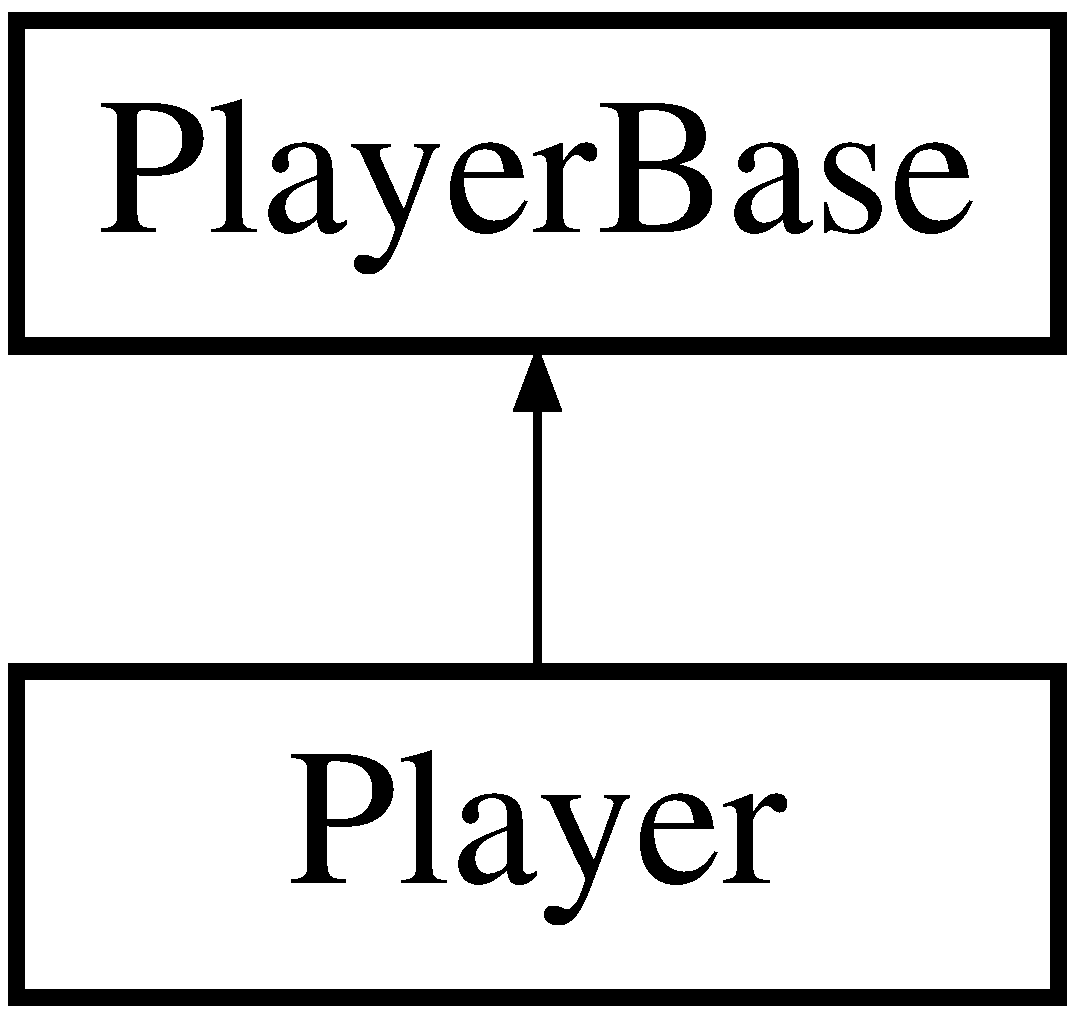
\includegraphics[height=2.000000cm]{classPlayer}
\end{center}
\end{figure}
\subsection*{Public Member Functions}
\begin{DoxyCompactItemize}
\item 
\hyperlink{classPlayer_a4d028f546b1dea57a0c0d76fc3a0de55}{Player} (const std\-::string \&name, Q\-String color, const std\-::vector$<$ std\-::shared\-\_\-ptr$<$ Course\-::\-Game\-Object $>$ $>$ objects=\{\})
\begin{DoxyCompactList}\small\item\em Constructor for the class. \end{DoxyCompactList}\item 
bool \hyperlink{classPlayer_a2ca3b33712ae6ef5be021a89c4f0b812}{modify\-Resource} (const Course\-::\-Basic\-Resource \&resource, const int \&amount)
\begin{DoxyCompactList}\small\item\em Modifies a players resource (by addition) \end{DoxyCompactList}\item 
bool \hyperlink{classPlayer_a8f2a8cb9cdda8bb195b90172d2b4e0e9}{modify\-Resources} (const Course\-::\-Resource\-Map \&resources)
\begin{DoxyCompactList}\small\item\em Modifies a players resources (by addition) \end{DoxyCompactList}\item 
Course\-::\-Resource\-Map \hyperlink{classPlayer_a7d91805e49dd4f33f9696c0dc6216993}{get\-Resources} () const 
\begin{DoxyCompactList}\small\item\em Returns the player's resources. \end{DoxyCompactList}\item 
const Q\-String \hyperlink{classPlayer_a228fc8436183fc5e60a8a5c5f1973607}{get\-Color} () const 
\begin{DoxyCompactList}\small\item\em Returns the player's color. \end{DoxyCompactList}\end{DoxyCompactItemize}


\subsection{Detailed Description}
The \hyperlink{classPlayer}{Player} class represents a player in the game. 

\hyperlink{classPlayer}{Player} has a name, color and ownership to Game\-Objects 

\subsection{Constructor \& Destructor Documentation}
\hypertarget{classPlayer_a4d028f546b1dea57a0c0d76fc3a0de55}{\index{Player@{Player}!Player@{Player}}
\index{Player@{Player}!Player@{Player}}
\subsubsection[{Player}]{\setlength{\rightskip}{0pt plus 5cm}Player\-::\-Player (
\begin{DoxyParamCaption}
\item[{const std\-::string \&}]{name, }
\item[{Q\-String}]{color, }
\item[{const std\-::vector$<$ std\-::shared\-\_\-ptr$<$ Course\-::\-Game\-Object $>$ $>$}]{objects = {\ttfamily \{\}}}
\end{DoxyParamCaption}
)}}\label{classPlayer_a4d028f546b1dea57a0c0d76fc3a0de55}


Constructor for the class. 


\begin{DoxyParams}{Parameters}
{\em name} & A std\-::string for player's name \\
\hline
{\em color} & \hyperlink{classPlayer}{Player}'s color in the game as a string \\
\hline
{\em objects} & (optional) A std\-::vector of shared-\/pointers to Game\-Objects. \\
\hline
\end{DoxyParams}


\subsection{Member Function Documentation}
\hypertarget{classPlayer_a228fc8436183fc5e60a8a5c5f1973607}{\index{Player@{Player}!get\-Color@{get\-Color}}
\index{get\-Color@{get\-Color}!Player@{Player}}
\subsubsection[{get\-Color}]{\setlength{\rightskip}{0pt plus 5cm}const Q\-String Player\-::get\-Color (
\begin{DoxyParamCaption}
{}
\end{DoxyParamCaption}
) const}}\label{classPlayer_a228fc8436183fc5e60a8a5c5f1973607}


Returns the player's color. 

\begin{DoxyReturn}{Returns}
Qstring that tells the player's color 
\end{DoxyReturn}
\hypertarget{classPlayer_a7d91805e49dd4f33f9696c0dc6216993}{\index{Player@{Player}!get\-Resources@{get\-Resources}}
\index{get\-Resources@{get\-Resources}!Player@{Player}}
\subsubsection[{get\-Resources}]{\setlength{\rightskip}{0pt plus 5cm}Course\-::\-Resource\-Map Player\-::get\-Resources (
\begin{DoxyParamCaption}
{}
\end{DoxyParamCaption}
) const}}\label{classPlayer_a7d91805e49dd4f33f9696c0dc6216993}


Returns the player's resources. 

\begin{DoxyReturn}{Returns}
Resource\-Map containing players resources 
\end{DoxyReturn}
\hypertarget{classPlayer_a2ca3b33712ae6ef5be021a89c4f0b812}{\index{Player@{Player}!modify\-Resource@{modify\-Resource}}
\index{modify\-Resource@{modify\-Resource}!Player@{Player}}
\subsubsection[{modify\-Resource}]{\setlength{\rightskip}{0pt plus 5cm}bool Player\-::modify\-Resource (
\begin{DoxyParamCaption}
\item[{const Course\-::\-Basic\-Resource \&}]{resource, }
\item[{const int \&}]{amount}
\end{DoxyParamCaption}
)}}\label{classPlayer_a2ca3b33712ae6ef5be021a89c4f0b812}


Modifies a players resource (by addition) 


\begin{DoxyParams}{Parameters}
{\em resource} & A Basic\-Resource type that is modified \\
\hline
{\em amount} & Amount of that resource \\
\hline
\end{DoxyParams}
\begin{DoxyReturn}{Returns}
Bool that tells if the operation was successful 
\end{DoxyReturn}
\hypertarget{classPlayer_a8f2a8cb9cdda8bb195b90172d2b4e0e9}{\index{Player@{Player}!modify\-Resources@{modify\-Resources}}
\index{modify\-Resources@{modify\-Resources}!Player@{Player}}
\subsubsection[{modify\-Resources}]{\setlength{\rightskip}{0pt plus 5cm}bool Player\-::modify\-Resources (
\begin{DoxyParamCaption}
\item[{const Course\-::\-Resource\-Map \&}]{resources}
\end{DoxyParamCaption}
)}}\label{classPlayer_a8f2a8cb9cdda8bb195b90172d2b4e0e9}


Modifies a players resources (by addition) 


\begin{DoxyParams}{Parameters}
{\em resources} & A Resource\-Map that is added to players resources \\
\hline
\end{DoxyParams}
\begin{DoxyReturn}{Returns}
Bool that tells if the operation was successful 
\end{DoxyReturn}


The documentation for this class was generated from the following files\-:\begin{DoxyCompactItemize}
\item 
player.\-h\item 
player.\-cpp\end{DoxyCompactItemize}

%--- End generated contents ---

% Index
\newpage
\phantomsection
\addcontentsline{toc}{part}{Index}
\printindex

\end{document}
